\documentclass[11pt]{article}
\usepackage[utf8]{inputenc}
\usepackage[spanish,es-tabla,es-nodecimaldot]{babel}

% Paquetess

\usepackage{amsmath}
\usepackage{amsthm}
\usepackage{amsfonts}
\usepackage{amssymb}
\usepackage{makeidx}
\usepackage{graphicx}
\usepackage{lmodern}
\usepackage[dvipsnames]{xcolor} 
\usepackage{fancyhdr}
\usepackage{geometry}
\usepackage{lastpage}		
\usepackage{array}			 % Para fjar tamaño de columnas
\usepackage{tikz}
\usepackage{subcaption}
\usepackage{caption}
\usepackage{pgfplots} % Para controlar la perspectiva
\RequirePackage{siunitx}
\usepackage{extramarks} % Para poder usar firstleftmarks
\usepackage[version=4]{mhchem} % Para poder usar formulas de reacciones nucleares
\usepackage{chemfig}
\usepackage{xcolor}
\RequirePackage[most]{tcolorbox}
\usepackage{enumitem}
\usepackage{physics}
%\usepackage{background}
\usepackage{eso-pic} % Para insertar imágenes de fondo específicas
\usepackage[absolute,overlay]{textpos} % Paquete para colocar elementos en posiciones absolutas
\usepackage{wrapfig}
\usepackage{booktabs}

\setlength{\parindent}{0pt} % Elimina la sangría
\newtcolorbox{mybox}{colback=black!5!white,
	colframe=black!75!black}

\newtcolorbox{Anotacion}{colback=red!5!white,
	colframe=red!75!red}


%##############################################################################
%######### Ponemos el decimal con . ###########################################
%##############################################################################

\sisetup{output-decimal-marker={.},
	% exponentes ------------------------
	exponent-mode=threshold,
	exponent-thresholds=-3:2, % non usar exponentes 10^{-2,-1, 0, 1}
	% redondear -------------------------
	% round-mode=figures, % cifras sig
	% round-mode=places, % cantos decimales
	round-mode=uncertainty, % cifras sig da incerteza (necesario usar erro)
	round-precision=2,
	uncertainty-mode = separate,
	print-unity-mantissa=false,
	% unidades --------------------------
	inter-unit-product = \ensuremath{{}\cdot{}}, % separacion entre unidades
	% per-mode=power-positive-first, % so furrula con metodo interpretado puro
	inline-per-mode=single-symbol,
	display-per-mode=fraction,
}

%##############################################################################
%######### Para codigo python #################################################
%##############################################################################

\definecolor{codegreen}{rgb}{0,0.6,0}
\definecolor{codegray}{rgb}{0.5,0.5,0.5}
\definecolor{codepurple}{rgb}{0.58,0,0.82}

\usepackage{listings}


%\lstdefinestyle{mystyle}{	backgroundcolor=\color{backcolour},   	commentstyle=\color{codegreen},	keywordstyle=\color{magenta},	numberstyle=\tiny\color{codegray},	stringstyle=\color{codepurple},	basicstyle=\ttfamily\footnotesize,	breakatwhitespace=false,         	breaklines=true,                 	captionpos=b,                    	keepspaces=true,                 	numbers=left,                    	numbersep=5pt,                  	showspaces=false,                	showstringspaces=false,	showtabs=false,                  	tabsize=2}

%\lstset{style=mystyle}
%\usepackage{background}     % Para manejar el fondo

%%%%%%%%%%%%%%%%%%%%%%%%%%%%%%%%%%%%%%%%%%
%%%%%%%%%%%%%%%%%% BIBLIOGRAFIA %%%%%%%%%%
%%%%%%%%%%%%%%%%%%%%%%%%%%%%%%%%%%%%%%%%%%


\usepackage{biblatex} %Imports biblatex package
\addbibresource{sample.bib} %Import the bibliography file

%##############################################################################
%######### Tipo de fuente #################################################
%##############################################################################

\usepackage{newtxtext,newtxmath} % Cambia la fuente (pero mola)
%\usepackage{kpfonts}

%\usepackage{helvet} 
%\renewcommand{\familydefault}{\sfdefault}.

%\usepackage{fontspec} % Paquete necesario para seleccionar fuentes
%\setmainfont{Verdana} % Cambia la fuente principal a Verdana


%##############################################################################
%######### Geometría #################################################
%##############################################################################

\geometry{a4paper, total={152mm,237mm}, left=31mm, top=30mm}



%##############################################################################
%######### Formatos capítulo #################################################
%##############################################################################

%\usepackage[lmodern]{quotchap}
%\usepackage[options]{fncychap}
% Configuración de la imagen de fondo solo para la portada



%##############################################################################
%######### Hiperreferenias #################################################
%##############################################################################


\usepackage[colorlinks=true, linkcolor=RoyalBlue, citecolor=ForestGreen, urlcolor=BrickRed]{hyperref} % Crea las
\usepackage[nameinlink]{cleveref}
\crefname{figure}{fig.}{Figs.}

%##############################################################################
%######### Formato de pagina #################################################
%##############################################################################

\pagestyle{fancy}
\fancyhf{} % Limpia encabezados y pies
\fancyhead[L]{\small \textbf{Memoria Resistividad de Placas}}    % Encabezado izquierdo
\fancyhead[R]{\small \textbf{Daniel Vázquez Lago}}     % Encabezado derecho
\fancyfoot[C]{\thepage}      % Pie de página centrado con el número de página
\renewcommand{\headrulewidth}{0.4pt}  % Grosor de la línea del encabezado
\renewcommand{\footrulewidth}{0pt}    % Sin línea en el pie



%##############################################################################
%#########  Modificar caption #################################################
%##############################################################################

\usepackage[font=small, justification=centering]{caption}  % Configura las captions



%##############################################################################
%######### Comandos propios #################################################
%##############################################################################


\newcommand{\parentesis}[1]{\left( #1  \right)}
\newcommand{\parciales}[2]{\frac{\partial #1}{\partial #2}}
\newcommand{\pparciales}[2]{\parentesis{\parciales{#1}{#2}}}
\newcommand{\ccorchetes}[1]{\left[ #1  \right]}
\newcommand{\D}{\mathrm{d}}
\newcommand{\derivadas}[2]{\frac{\D #1}{\D #2}}

\newcommand{\tquad}{\quad \quad \quad}
%\newcommand{\vnabla}{\vec{\nabla}}

\newcommand{\Ocal}{\mathcal{O}}
\newcommand{\Jcal}{\mathcal{J}}
\newcommand{\Mcal}{\mathcal{M}}
\newcommand{\Fcal}{\mathcal{F}}
\newcommand{\Hcal}{\mathcal{H}}
\newcommand{\Ecal}{\mathcal{E}}
\newcommand{\Ncal}{\mathcal{N}}

\newcommand{\cmm}{\text{cm}^{-1}}
\newcommand{\fcc}{\textit{fcc}}
\newcommand{\bcc}{\textit{bcc}}
\renewcommand{\sc}{\textit{sc}}
\newcommand{\hcp}{\textit{hcp}}


\newcommand{\PZB}{\text{{\tiny PZB}}}
\newcommand{\gap}{\text{{\tiny gap}}}
\newcommand{\SZB}{\text{{\tiny SZB}}}
\newcommand{\inicial}{\text{{\tiny inicial}}}
\newcommand{\final}{\text{{\tiny final}}}
\newcommand{\atomico}{\text{{\tiny atómico}}}

\newcommand{\arctanh}{\text{{arctanh}}}



\newcommand{\Namas}{\text{Na}^+}
\newcommand{\Clmenos}{\text{Cl}^-}

\newcommand{\cm}{\text{cm}}
\newcommand{\eV}{\text{eV}}

\newcommand{\arr}{\text{arr}}
\newcommand{\diff}{\text{diff}}

\newcommand{\er}{$^{\text{er}}$}
\newcommand{\cte}{\text{cte}}
\newcommand{\expo}{\text{exp}}
\newcommand{\simu}{\text{simu}}


% Comandos vectoriales

\newcommand{\an}{\mathbf{a}}
\newcommand{\bn}{\mathbf{b}}
\newcommand{\dn}{\mathbf{d}}
\newcommand{\fn}{\mathbf{f}}
\newcommand{\jn}{\mathbf{j}}
\newcommand{\kn}{\mathbf{k}}
\newcommand{\pn}{\mathbf{p}}
\newcommand{\qn}{\mathbf{q}}
\newcommand{\rn}{\mathbf{r}}
\newcommand{\sn}{\mathbf{s}}
\newcommand{\un}{\mathbf{u}}
\newcommand{\vn}{\mathbf{v}}
\newcommand{\xn}{\mathbf{x}}
\newcommand{\wn}{\mathbf{w}}
\newcommand{\yn}{\mathbf{y}}
\newcommand{\qndot}{\dot{\qn}}

\newcommand{\alphan}{\boldsymbol{\alpha}}
\newcommand{\sigman}{\boldsymbol{\sigma}}
\newcommand{\pin}{\boldsymbol{\pi}}
\newcommand{\rhon}{\boldsymbol{\rho}}
\newcommand{\epsilonn}{\boldsymbol{\epsilon}}
\newcommand{\omegan}{\boldsymbol{\omega}}
\newcommand{\mun}{\boldsymbol{\mu}}



\newcommand{\An}{\mathbf{A}}
\newcommand{\Bn}{\mathbf{B}}
\newcommand{\En}{\mathbf{E}}
\newcommand{\Fn}{\mathbf{F}}
\newcommand{\Jn}{\mathbf{J}}
\newcommand{\Hn}{\mathbf{H}}
\newcommand{\Gn}{\mathbf{G}}
\newcommand{\Kn}{\mathbf{K}}
\newcommand{\Ln}{\mathbf{L}}
\newcommand{\Mn}{\mathbf{M}}
\newcommand{\Pn}{\mathbf{P}}
%\newcommand{\Rn}{\mathbf{R}}
\newcommand{\Sn}{\mathbf{S}}
\newcommand{\Tn}{\mathbf{T}}
\newcommand{\In}{\mathbf{1}}
\newcommand{\Encal}{\boldsymbol{\mathcal{E}}}

\newcommand{\hnn}{\hat{\mathbf{n}}}
\newcommand{\hnr}{\hat{\mathbf{r}}}
\newcommand{\hnz}{\hat{\mathbf{z}}}
\newcommand{\hnv}{\hat{\mathbf{v}}}
\newcommand{\hnx}{\hat{\mathbf{x}}}
\newcommand{\hny}{\hat{\mathbf{y}}}
\newcommand{\hnu}{\hat{\mathbf{u}}}
\newcommand{\hnR}{\hat{\mathbf{R}}}
\newcommand{\hnp}{\hat{\mathbf{p}}}
\newcommand{\hnk}{\hat{\mathbf{k}}}
\newcommand{\hni}{\hat{\mathbf{i}}}
\newcommand{\hnj}{\hat{\mathbf{j}}}
\renewcommand{\hnk}{\hat{\mathbf{k}}}

 
\title{Memoria Tecnicas IV Sólido: Resistividad de Placas}
\author{Daniel Vázquez Lago}
\date{\today}




\begin{document}

\maketitle

\tableofcontents

\setlength{\parskip}{1.8mm}                         % Cambia el espacio entre párrafos

\newpage

\section{Objetivos}

El principal objetivo es determinar la resisitivdad eléctrica del material de la placa de espesor 1 mm, y luego identificar el metal. 

\section{Procedimiento a la medida}

Esta es la parte puramente experimental. Lo que hacemos es inyectar una corriente por dos terminales cualquiera (1,2,3,4), \cref{Fig:01}, midiendo la diferencia de voltaje por otras dos. Nostros realizamos 4 medidas de Intensidad-Voltaje (tal que $I\leq 4$ A y $V\leq 1$ mV) en 6 diferentes disposiciones. Realizar 4 medidas, que nosotros tomamos desde 1.5 A a 3.0 A con un intervalo de 0.5 A, es suficiente para comprobar que efectivamente es un material óhmico, que es la única exigencia que vamos a realizar para el análisis posterior. Dado que el cálculo de la resistividad se realiza con un solo valor del voltaje para cada disposición no será un problema tener pocas medidas (al memos en comparación con otras prácticas). 

\begin{figure}[h!] \centering
	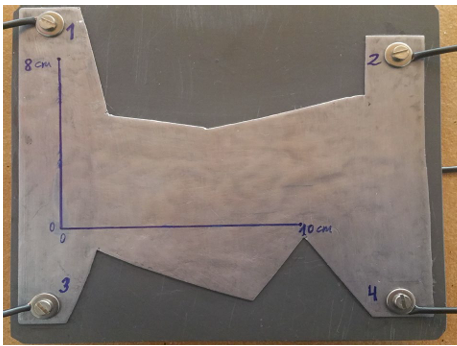
\includegraphics{Agros/placa prueba.png}
	\caption{imagen de la placa dentada que vamos a usar con los diferentes terminales.}
	\label{Fig:01}
\end{figure}
Como realizamos la digitalización o la simulación es un, ciertamente, innecesario, ya que todo lo que realizamos está en el guión de la práctica. 

\subsection{Notación de las disposiciones}

Para denotar las disposiciones de ahora en adelante vamos a usar el siguiente código. Denotamos por disposición a $I(a,b)V(c,d)$ donde $a,b,c,d$ son números del 1 al 4, que corresponderán a las entradas y salidas de voltaje. Por ejemplo, $I(1,4)V(2,3)$ indica que $I^+$ estaba en la terminal 1, $I^-$ en 4, $V^+$ en 2 y $V^-$ en 3 \cite{IvanCambon}.

\section{Material óhmico}

Como podemos ver en las gráficas los resultados obtenidos indican un comportamiento claramente lineal entre intensidad y voltaje. En las gráficas representamos los puntos experimentales y el ajuste lineal, con los parámetros incluidos en la propia gráfica tal que: 

\begin{equation}
	y(x) = p_0 + p_1 \cdot x
\end{equation}
concluyendo que efectivamente es un \textbf{material óhmico} y que por tanto podemos obtener $\sigma_{\exp}$ a través del desarrollo teórico. 

\section{Calculo de la resistivdad del material}

Como ya hemos indicado, nosotros vamos a medir voltajes para una entrada particular de intensidad, queriendo calcular la resisitivdad del material, por lo que la información importante será $(V_{\exp},\sigma_{\exp})$, siendo $\sigma_{\exp}$ la que queremos calcular. Los valores que nos va a dar la simulación son pares de $(V_{\simu},\sigma_{\simu}$) siendo la intensidad $I_{\exp}$ y $I_{\simu}$ iguales, en una experimental y en otra un parámetro que introducimos a mano. Dado que la ley de Ohm $V\varpropto \rho = 1 / \sigma$ que hemos comprobado que el material sigue:, podemos suponer que $V\times \sigma = \cte$, y por tanto se debe verificar que: 

\begin{equation}
	V_{\exp} \times \sigma_{\exp} = V_{\simu} \times \sigma_{\simu}
\end{equation}
tal que: 

\begin{equation}
	\sigma_{\exp} =  \frac{V_{\simu}}{V_{exp}} \times \sigma_{\simu}
\end{equation}
Recordamos que la \textbf{resistividad} $\sigma$ se mide en $[\Omega \cdot m]$ y que su inversa es la \textbf{conductividad} denotada por $\gamma$:

\begin{equation}
	\gamma = \frac{1}{\sigma}
\end{equation}
que se mide en $[S / m]$.

La intensidad que nosotros medimos en el lab no es igual al parámetro que nos pide agros. El funcionamiento de agros es un poco complicado, ya que modeliza una terminal como un círculo formado por 4 segmentos, de tal modo que nosotros tenemos que introducir la corriente por segmento, así pues el $I$ que vamos a introducir está divido por 4. Sin embargo todavía falta algo, agros no pide el valor de la intensidad $I$ en amperios, tenemos que darle el valor de la densidad de corriente $J [\unit{A/m^2}]$, por lo que vamos a introducir el valor de $I$ dividido entre 4 y por el espesor y el tamaño de uno de los segmentos. Por suerte el espesor $d$ nos lo dan en el guión y lo tomaremos por un valor constante sin incertidumbre:

\begin{equation}
	d = 1 \ \unit{mm}
\end{equation}
Dado que la longitud de cada segmento dependerá de la modelización, y eso variará en función de la parte de la práctica en la que estemos, ya que como veremos, es una de las grandes fuentes de incertidumbre. 



\section{Resultados}

Los resultados los evaluaremos disposición a disposición, ya que cada una de ellas tiene bastantes tablas y figuras, por lo que vemos conveniente usarlas todas juntas.  \newpage

\subsection{Disposición 1}


\begin{figure}[h!]\centering
\begin{subfigure}[b]{0.49\textwidth}
	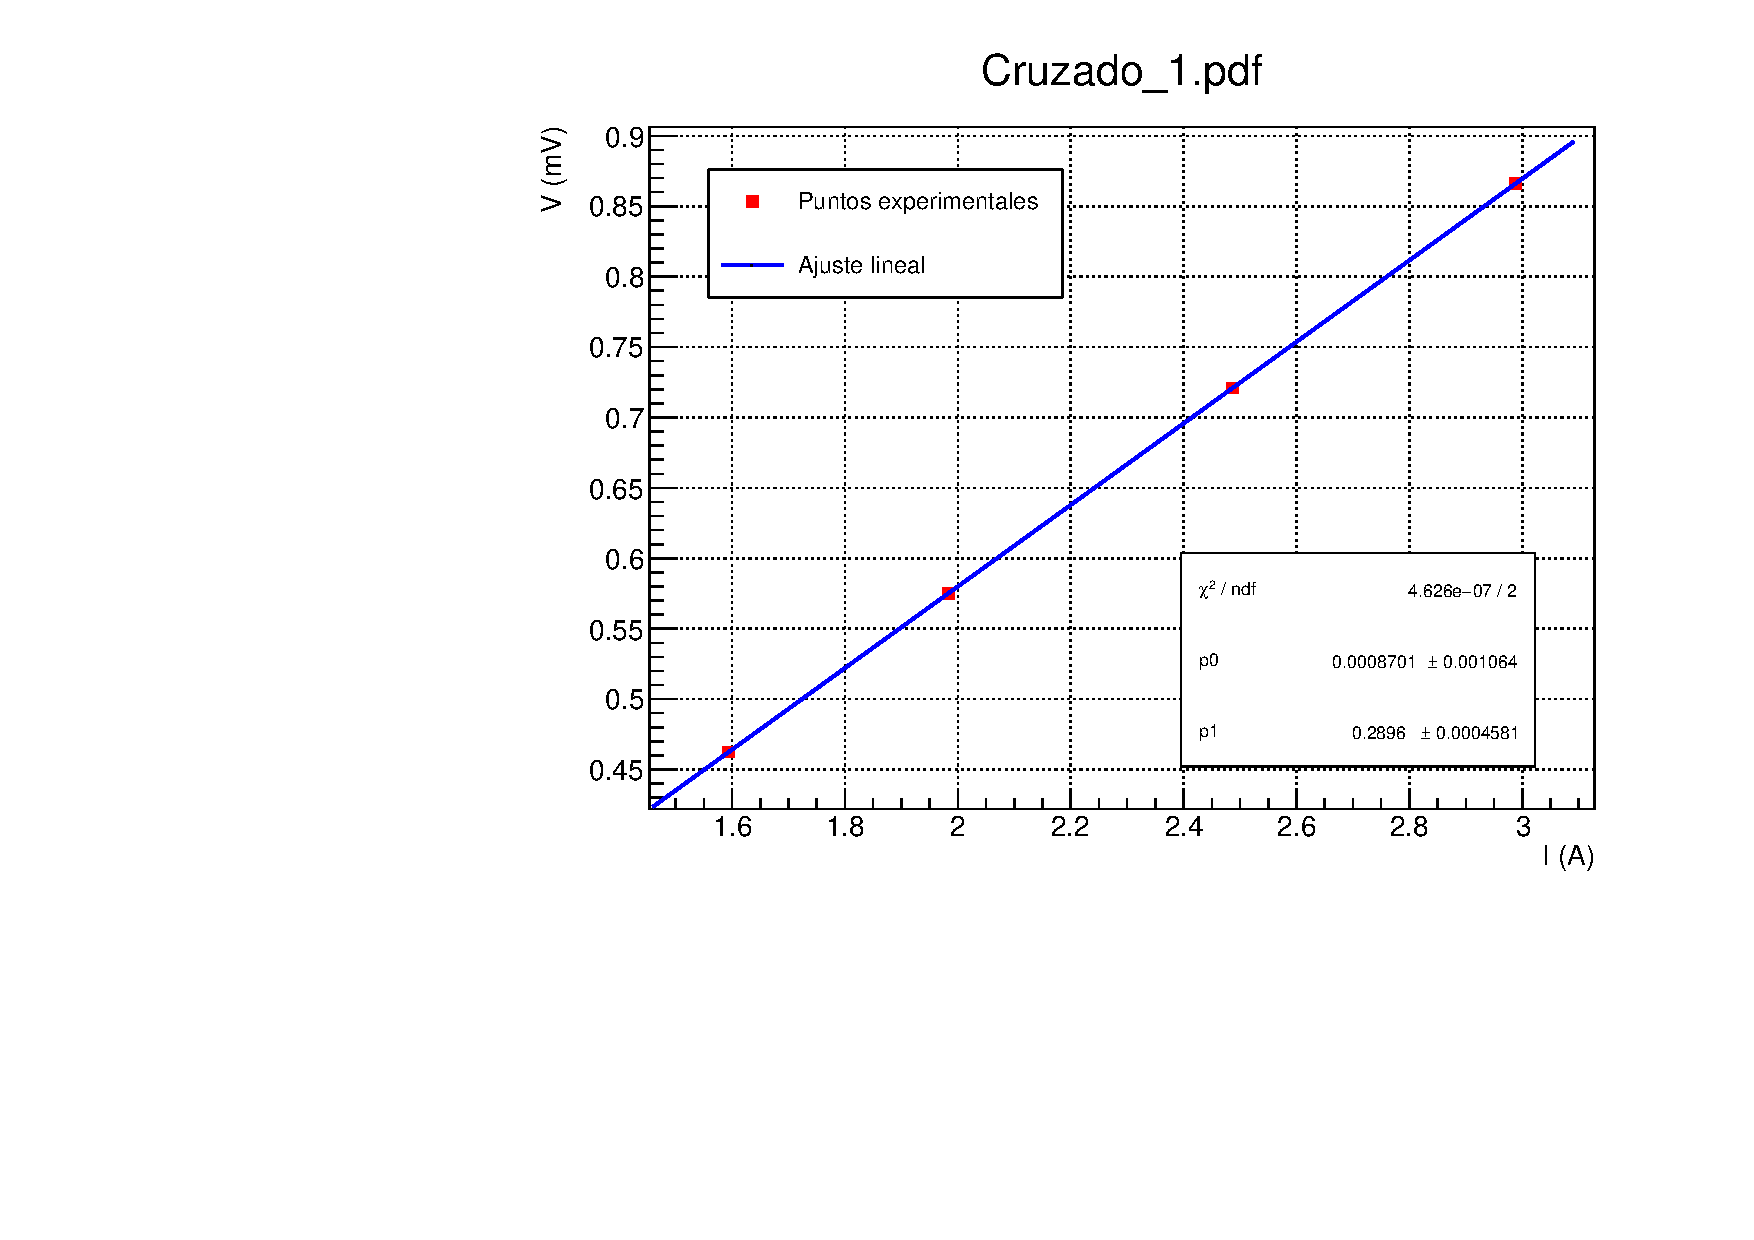
\includegraphics[width=1.05\linewidth]{Programas/Cruzado_1.pdf}
\end{subfigure} \hfill
\begin{subfigure}[b]{0.49\textwidth}
	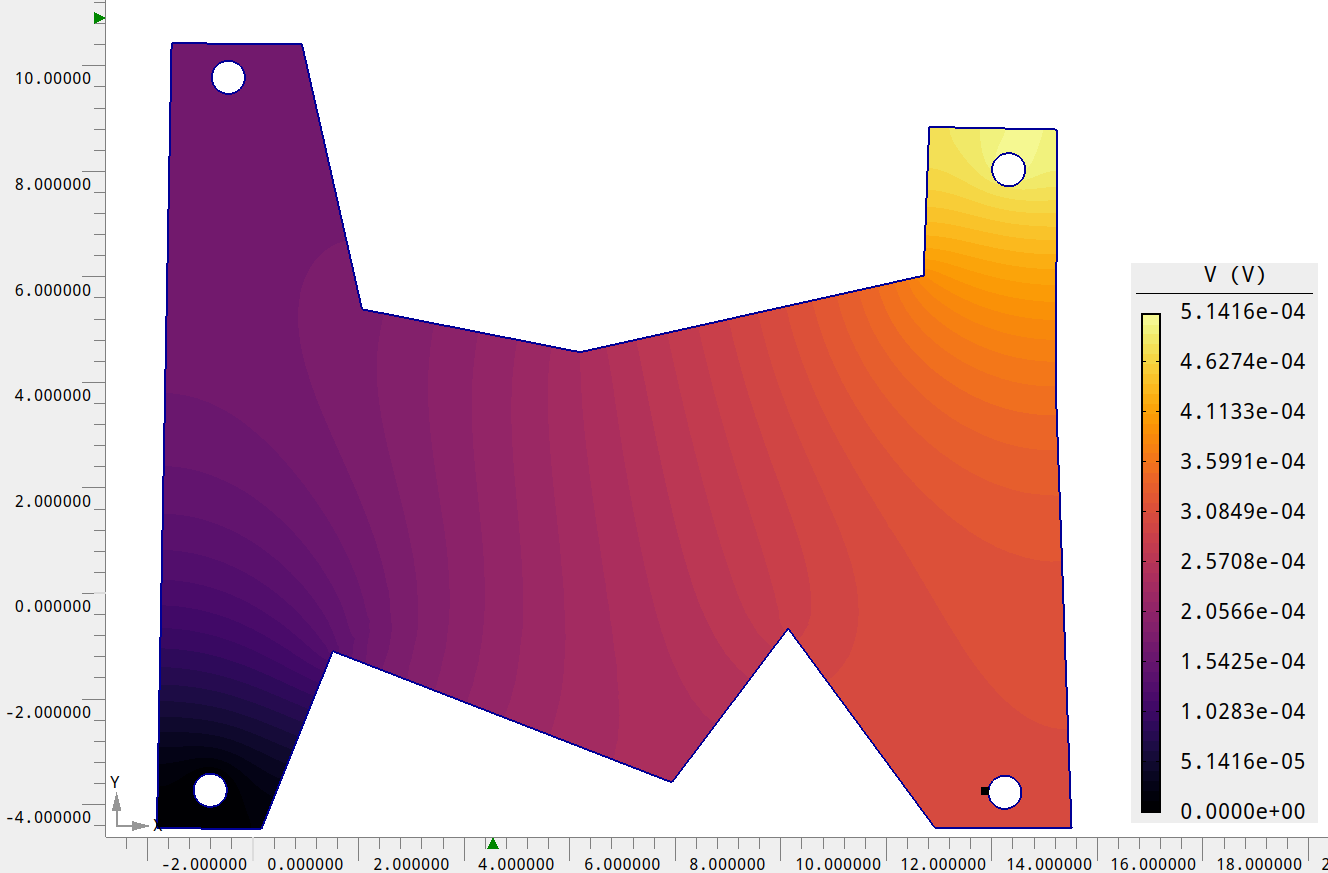
\includegraphics[width=1.05\linewidth]{Imagen Agros 1/Agros1.png}
\end{subfigure}
\end{figure}

Los valores experimentales tal que $\Delta V_{\exp}$, $I_{\exp}$ y $J_{\exp}$, usando que $r=$ tenemos: 

\begin{table}[h!]
    \centering
\begin{tabular}{ccc}
\toprule
$I$ [A] & $V$ [mV] & $J$ [A/cm$^2$] \\
\midrule
2.988 & 0.8660 & 15.184 \\
\bottomrule
\end{tabular}
    \caption{Tabla de la valores para la disposición 1 con $r=0.313$ cm}
    \label{Tab:VIJ_mini_1}
\end{table}


Dado que no podemos calcualr directamente $\Delta V_{\simu}$ ya que alrededor de las terminales varía un poco el voltaje (véase imagen) tal que mediremos varios $V_+$ y $V_-$ simulados, obteniendo una media (y su incertidumbre) y así $\Delta V_{\simu} = \overline{V}_+ - \overline{V}_{-} $. Así pues: 

\begin{table}[h!]
    \centering
\begin{tabular}{c|cccc|ccc}
\toprule
\midrule
$V_+$ [mV] & 0.08664 & 0.08663 & 0.08667 & 0.08664 & $\overline{V}_+$ & $\overline{V}_-$ & $dV$ \\
$V_-$ [mV] & \SI{1.537e-01}{} & \SI{1.535e-01}{} & \SI{1.536e-01}{} & \SI{1.538e-01}{} & \SI{1.537e-01}{} & \SI{8.665e-02}{} & \SI{6.700e-02}{} \\
\bottomrule
\end{tabular}
    \caption{Tabla de la valores para la disposición 1 de $V_+$ y $V_-$}
    \label{Tab:Vpn_1}
\end{table}

y el valor de la resistividad es: 

\begin{table}[h!]
    \centering
\begin{tabular}{cc}
\toprule
$\sigma$ [S/cm] & $\rho$ [$\Omega$cm] \\
\midrule
46386 & 0.0000216 \\
\bottomrule
\end{tabular}
    \caption{Tabla de la valores para la disposición 1 de $\sigma$ y $\rho $}
    \label{Tab:RS_1}
\end{table}


\newpage

\subsection{Disposición 2}


\begin{figure}[h!]\centering
\begin{subfigure}[b]{0.49\textwidth}
	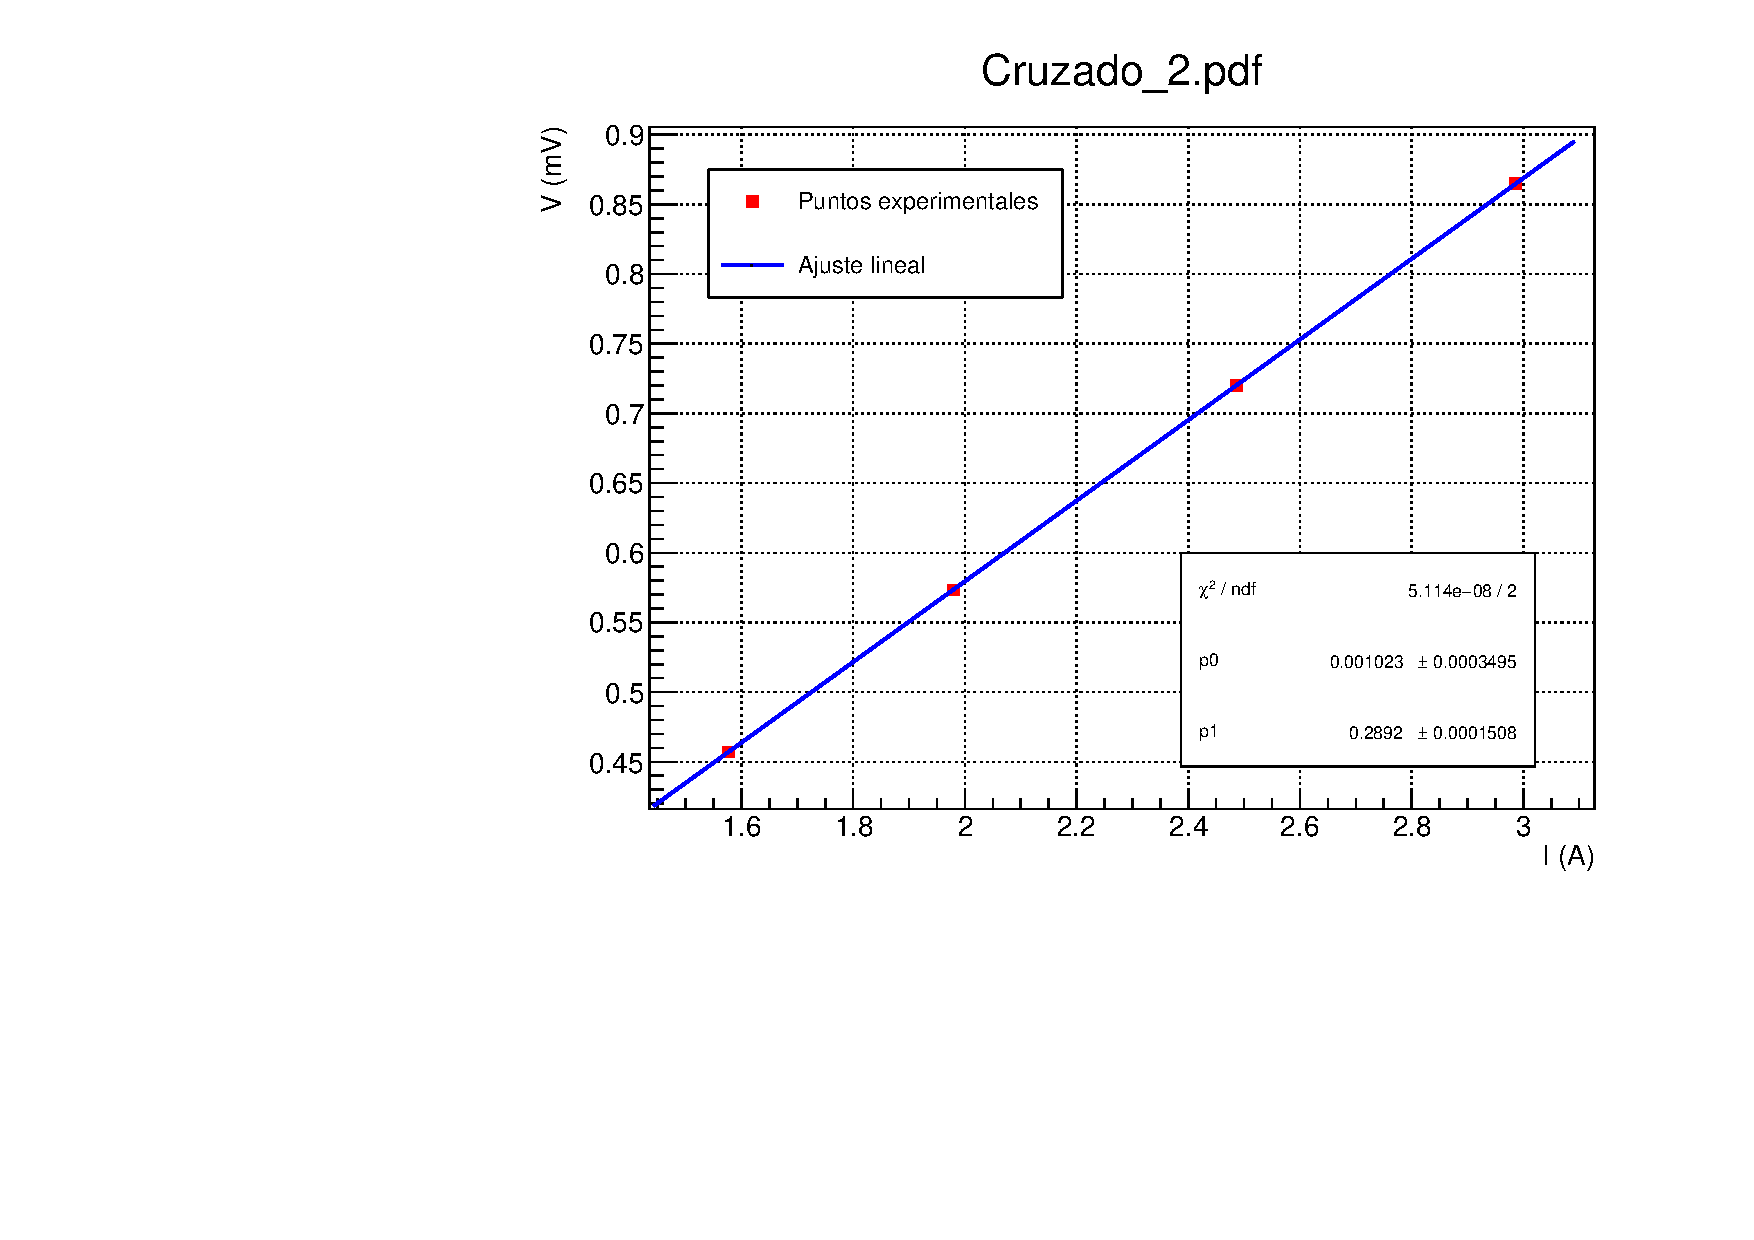
\includegraphics[width=1.05\linewidth]{Programas/Cruzado_2.pdf}
\end{subfigure} \hfill
\begin{subfigure}[b]{0.49\textwidth}
	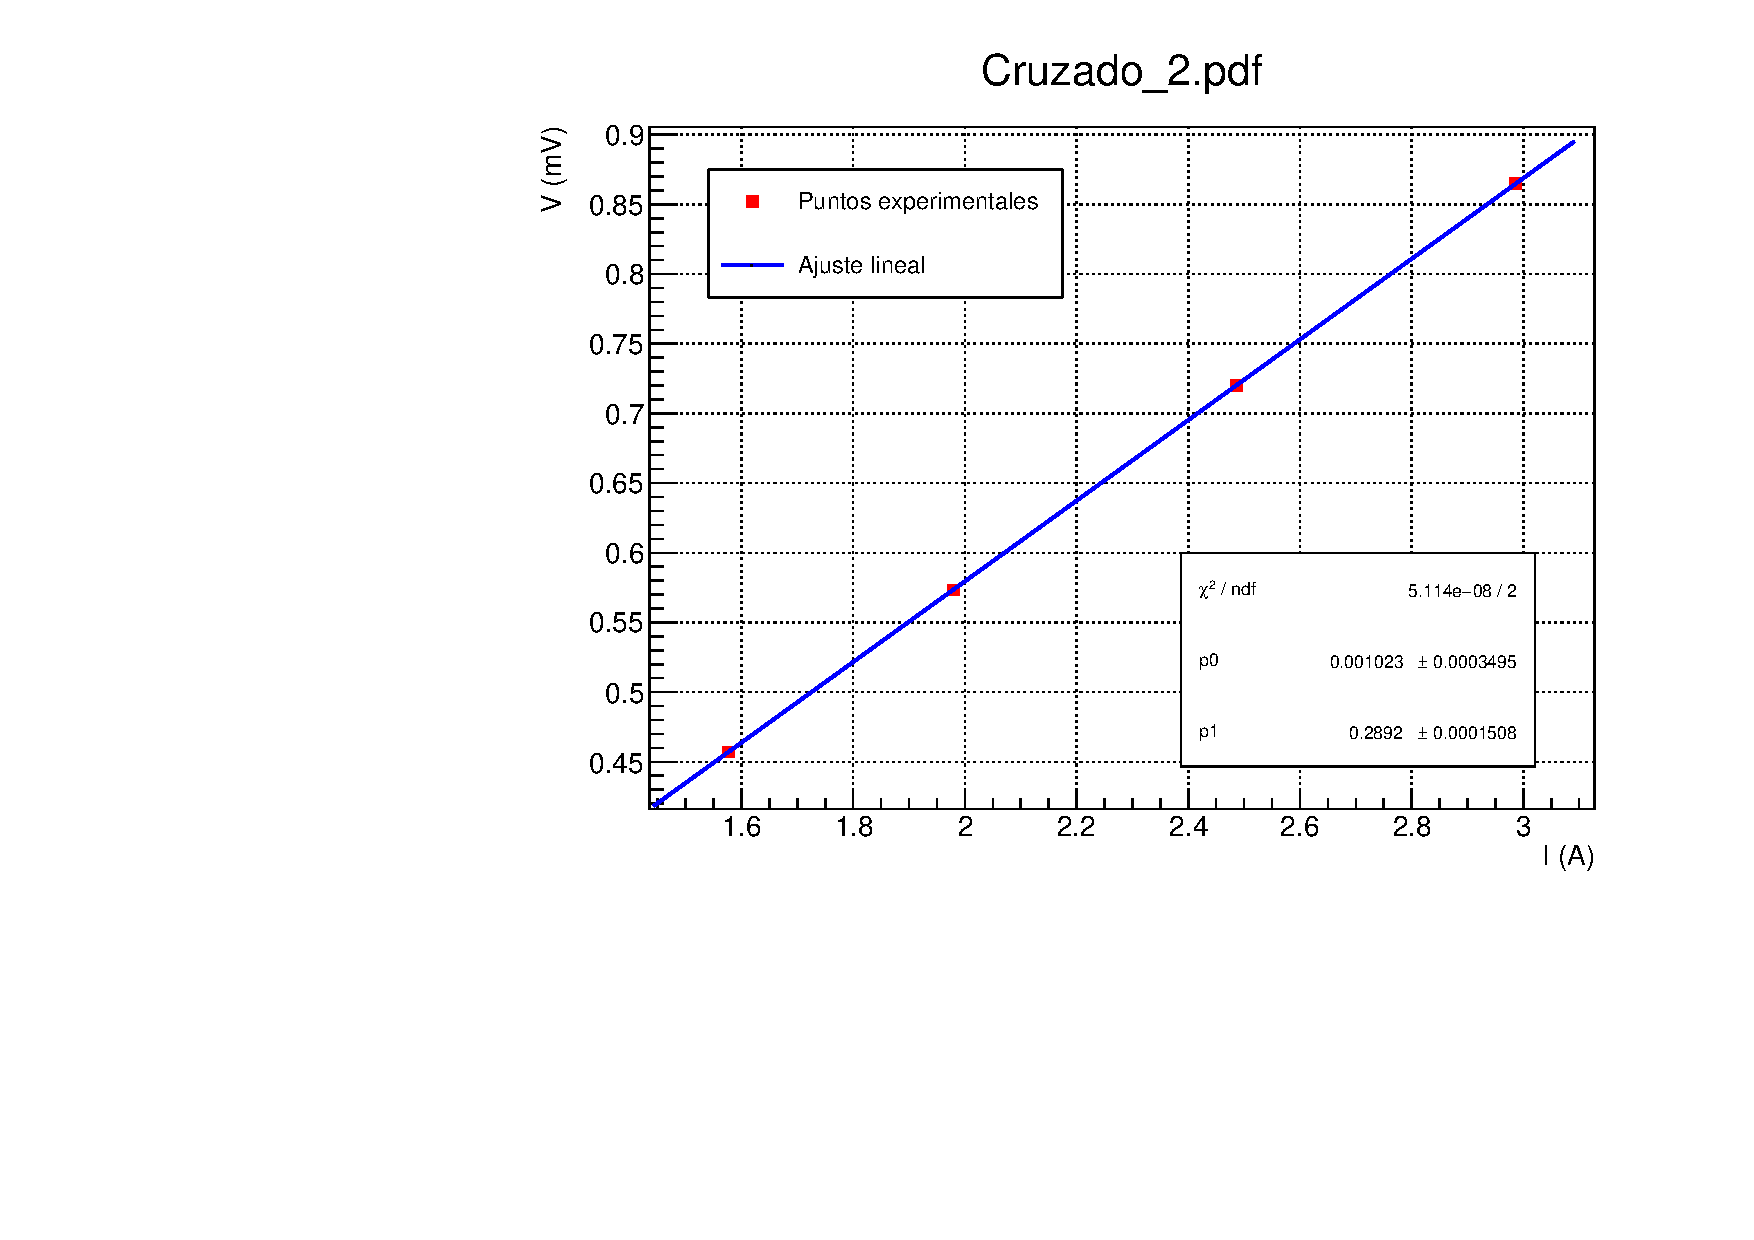
\includegraphics[width=1.05\linewidth]{Programas/Cruzado_2.pdf}
\end{subfigure}
\end{figure}


Los valores experimentales tal que $\Delta V_{\exp}$, $I_{\exp}$ y $J_{\exp}$, usando que $r=$ tenemos: 

\begin{table}[h!]
    \centering
\begin{tabular}{ccc}
\toprule
$I$ [A] & $V$ [mV] & $J$ [A/cm$^2$] \\
\midrule
2.986 & 0.8648 & 15.174 \\
\bottomrule
\end{tabular}
    \caption{Tabla de la valores para la disposición 2 con $r=0.313$ cm}
    \label{Tab:VIJ_mini_2}
\end{table}


Dado que no podemos calcualr directamente $\Delta V_{\simu}$ ya que alrededor de las terminales varía un poco el voltaje (véase imagen) tal que mediremos varios $V_+$ y $V_-$ simulados, obteniendo una media (y su incertidumbre) y así $\Delta V_{\simu} = \overline{V}_+ - \overline{V}_{-} $. Así pues: \\[1em]

Tal que $\Delta V_{\simu}$ es: \\[1em]

y luego, el valor de la resistividad es:

\newpage

\subsection{Disposición 3}

\begin{figure}[h!]\centering
\begin{subfigure}[b]{0.49\textwidth}
	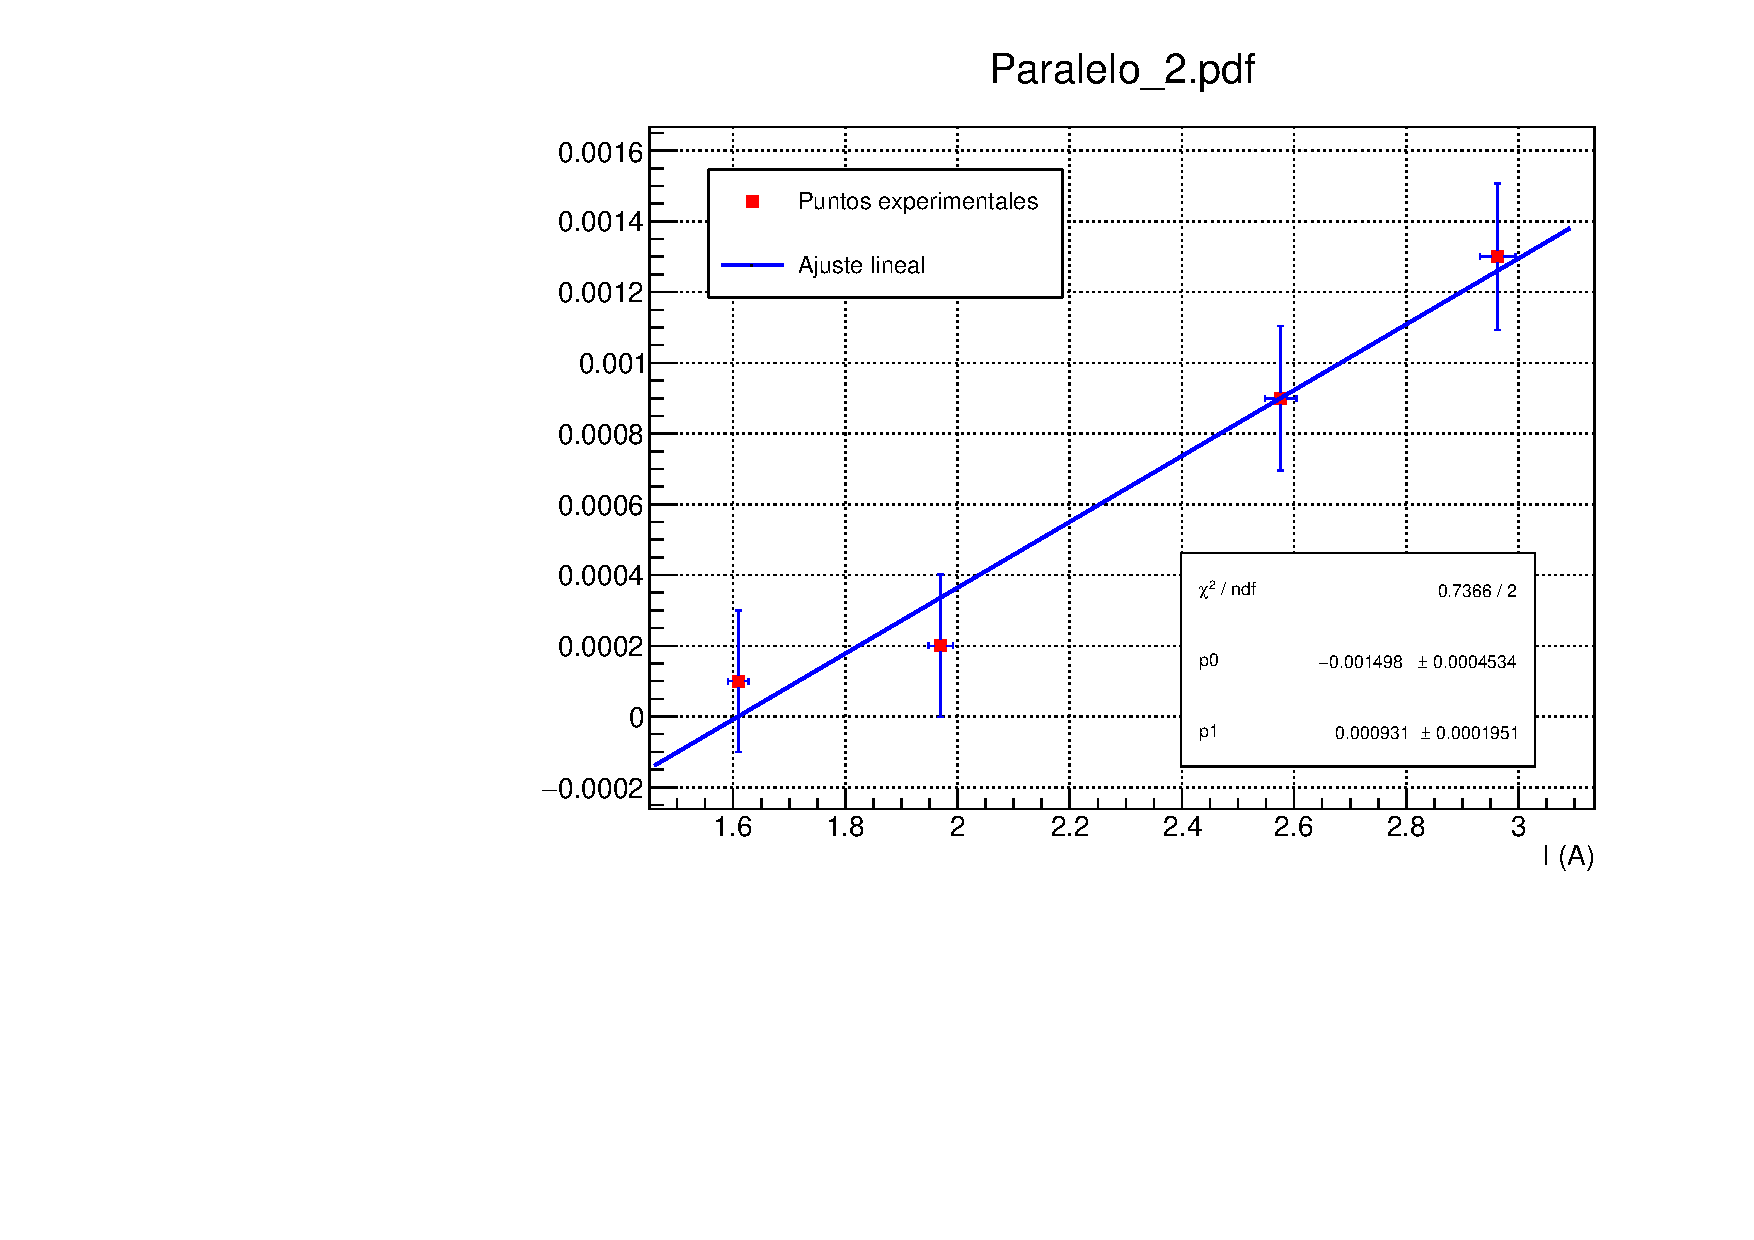
\includegraphics[width=1.05\linewidth]{Programas/Paralelo_2.pdf}
\end{subfigure} \hfill
\begin{subfigure}[b]{0.49\textwidth}
	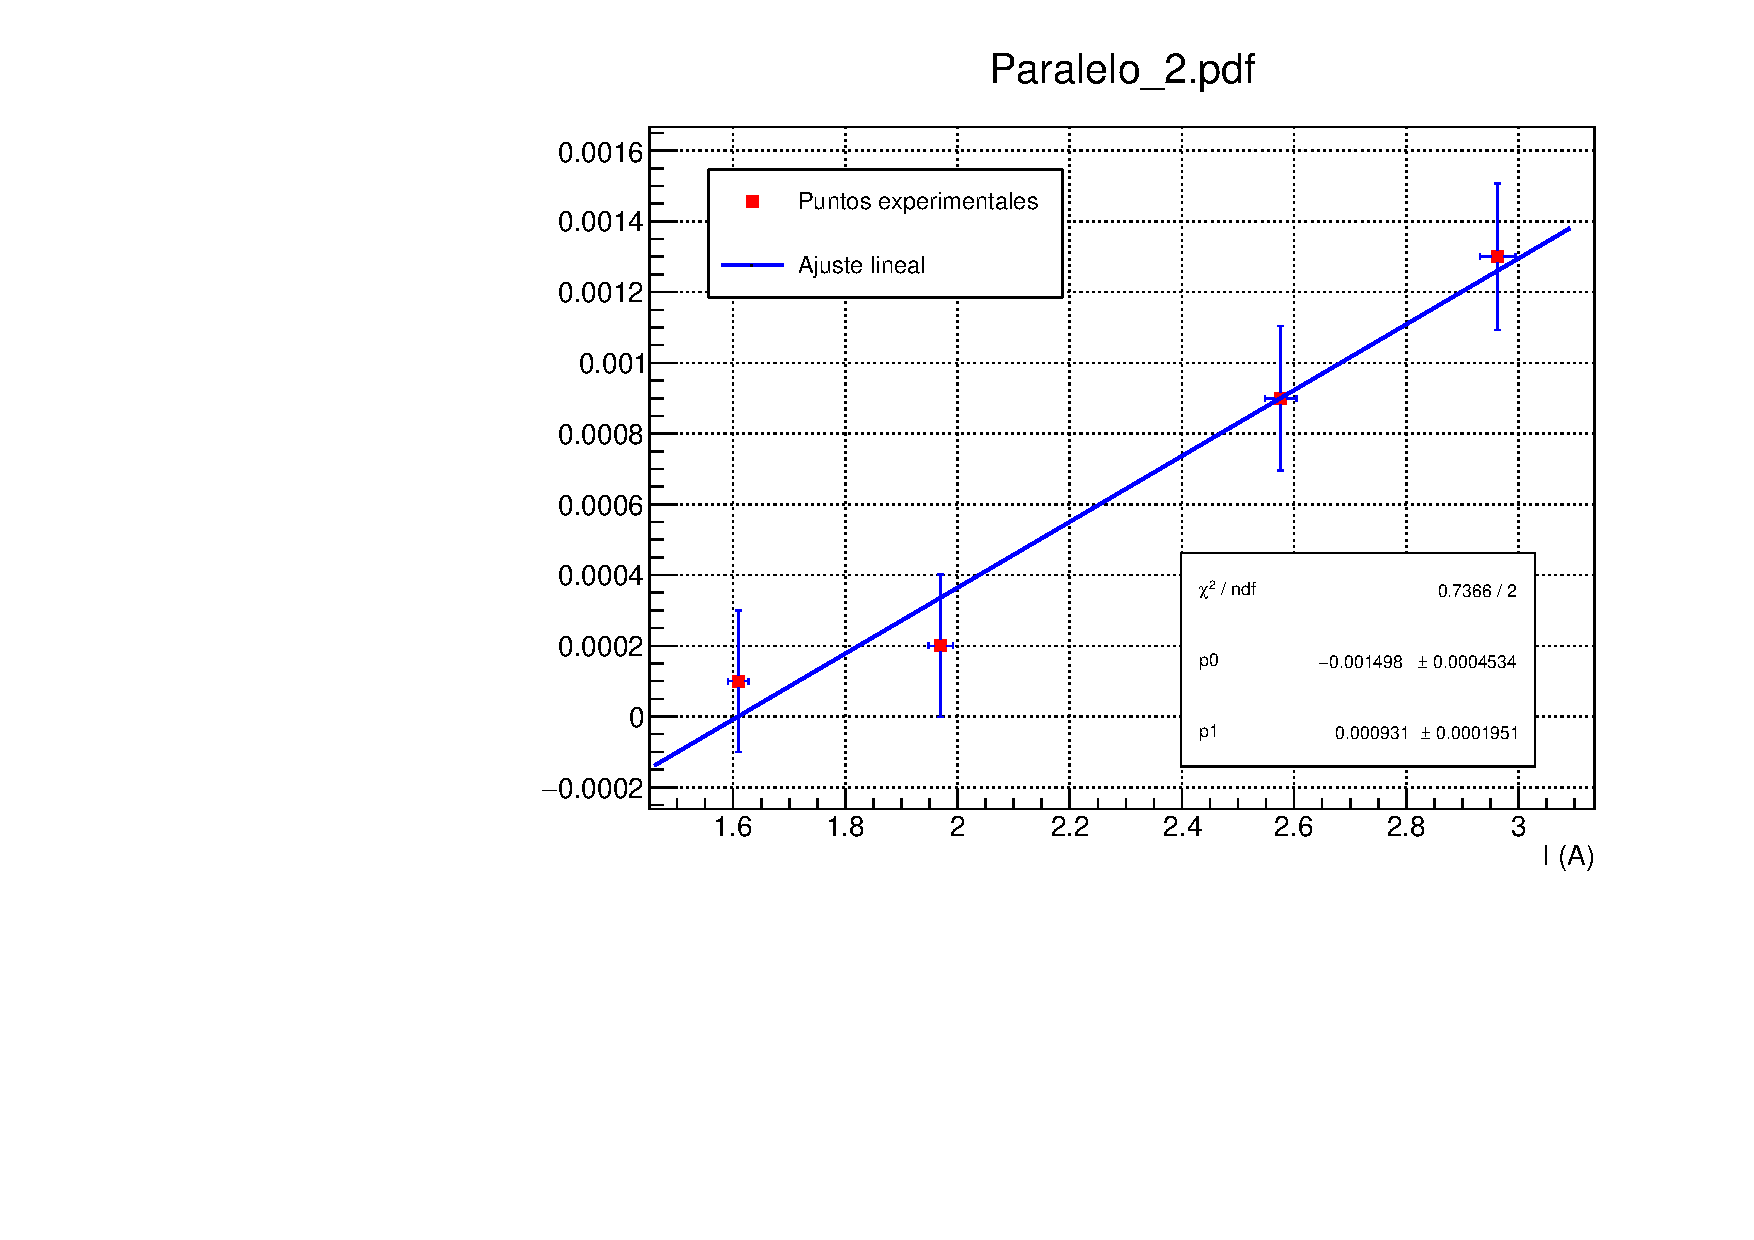
\includegraphics[width=1.05\linewidth]{Programas/Paralelo_2.pdf}
\end{subfigure}
\end{figure}


Los valores experimentales tal que $\Delta V_{\exp}$, $I_{\exp}$ y $J_{\exp}$, usando que $r=$ tenemos: 

\begin{table}[h!]
    \centering
\begin{tabular}{ccc}
\toprule
$I$ [A] & $V$ [mV] & $J$ [A/cm$^2$] \\
\midrule
3.051 & 0.0022 & 15.504 \\
\bottomrule
\end{tabular}
    \caption{Tabla de la valores para la disposición 3 con $r=0.313$ cm}
    \label{Tab:VIJ_mini_3}
\end{table}


Dado que no podemos calcualr directamente $\Delta V_{\simu}$ ya que alrededor de las terminales varía un poco el voltaje (véase imagen) tal que mediremos varios $V_+$ y $V_-$ simulados, obteniendo una media (y su incertidumbre) y así $\Delta V_{\simu} = \overline{V}_+ - \overline{V}_{-} $. Así pues: \\[1em]

Tal que $\Delta V_{\simu}$ es: \\[1em]

y luego, el valor de la resistividad es:


\newpage

\subsection{Disposición 4}

\begin{figure}[h!]\centering
	\begin{subfigure}[b]{0.49\textwidth}
		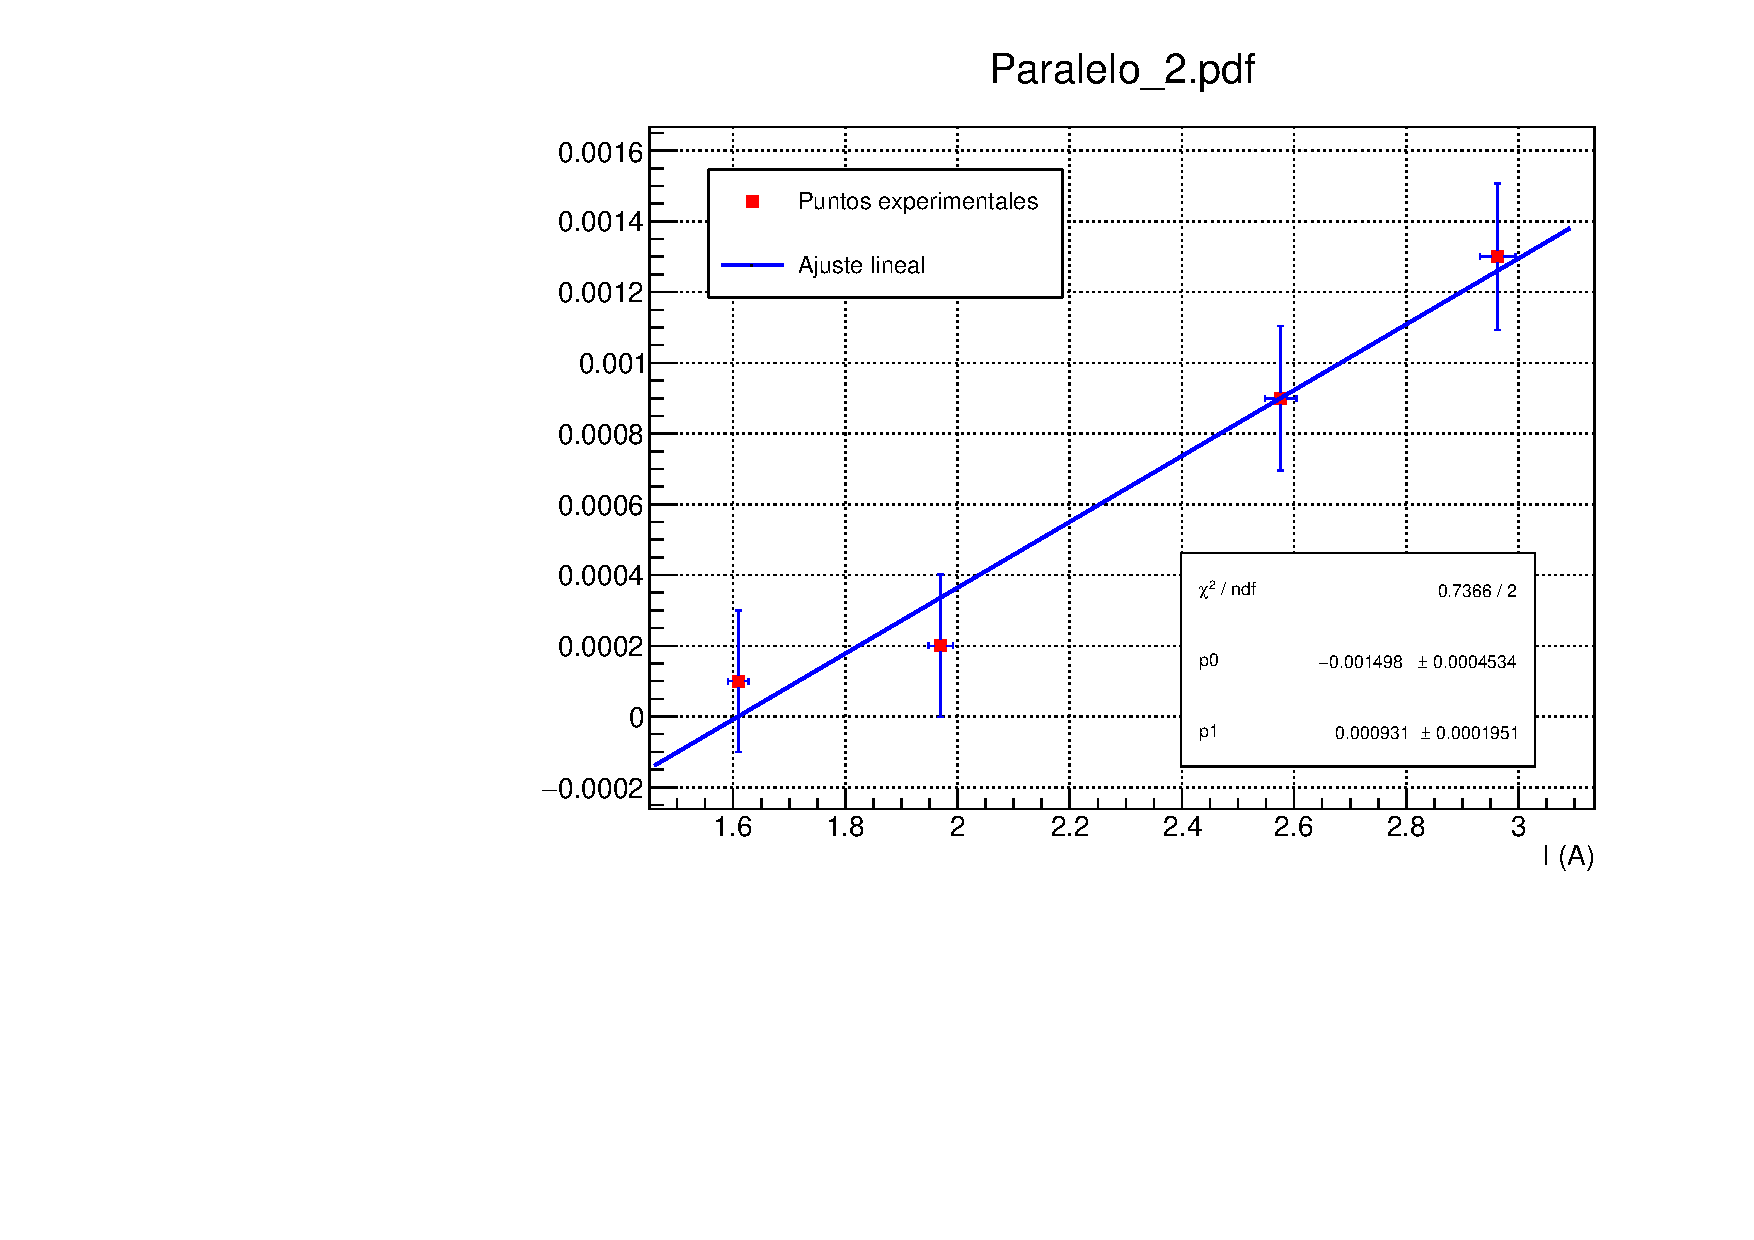
\includegraphics[width=1.05\linewidth]{Programas/Paralelo_2.pdf}
	\end{subfigure} \hfill
	\begin{subfigure}[b]{0.49\textwidth}
		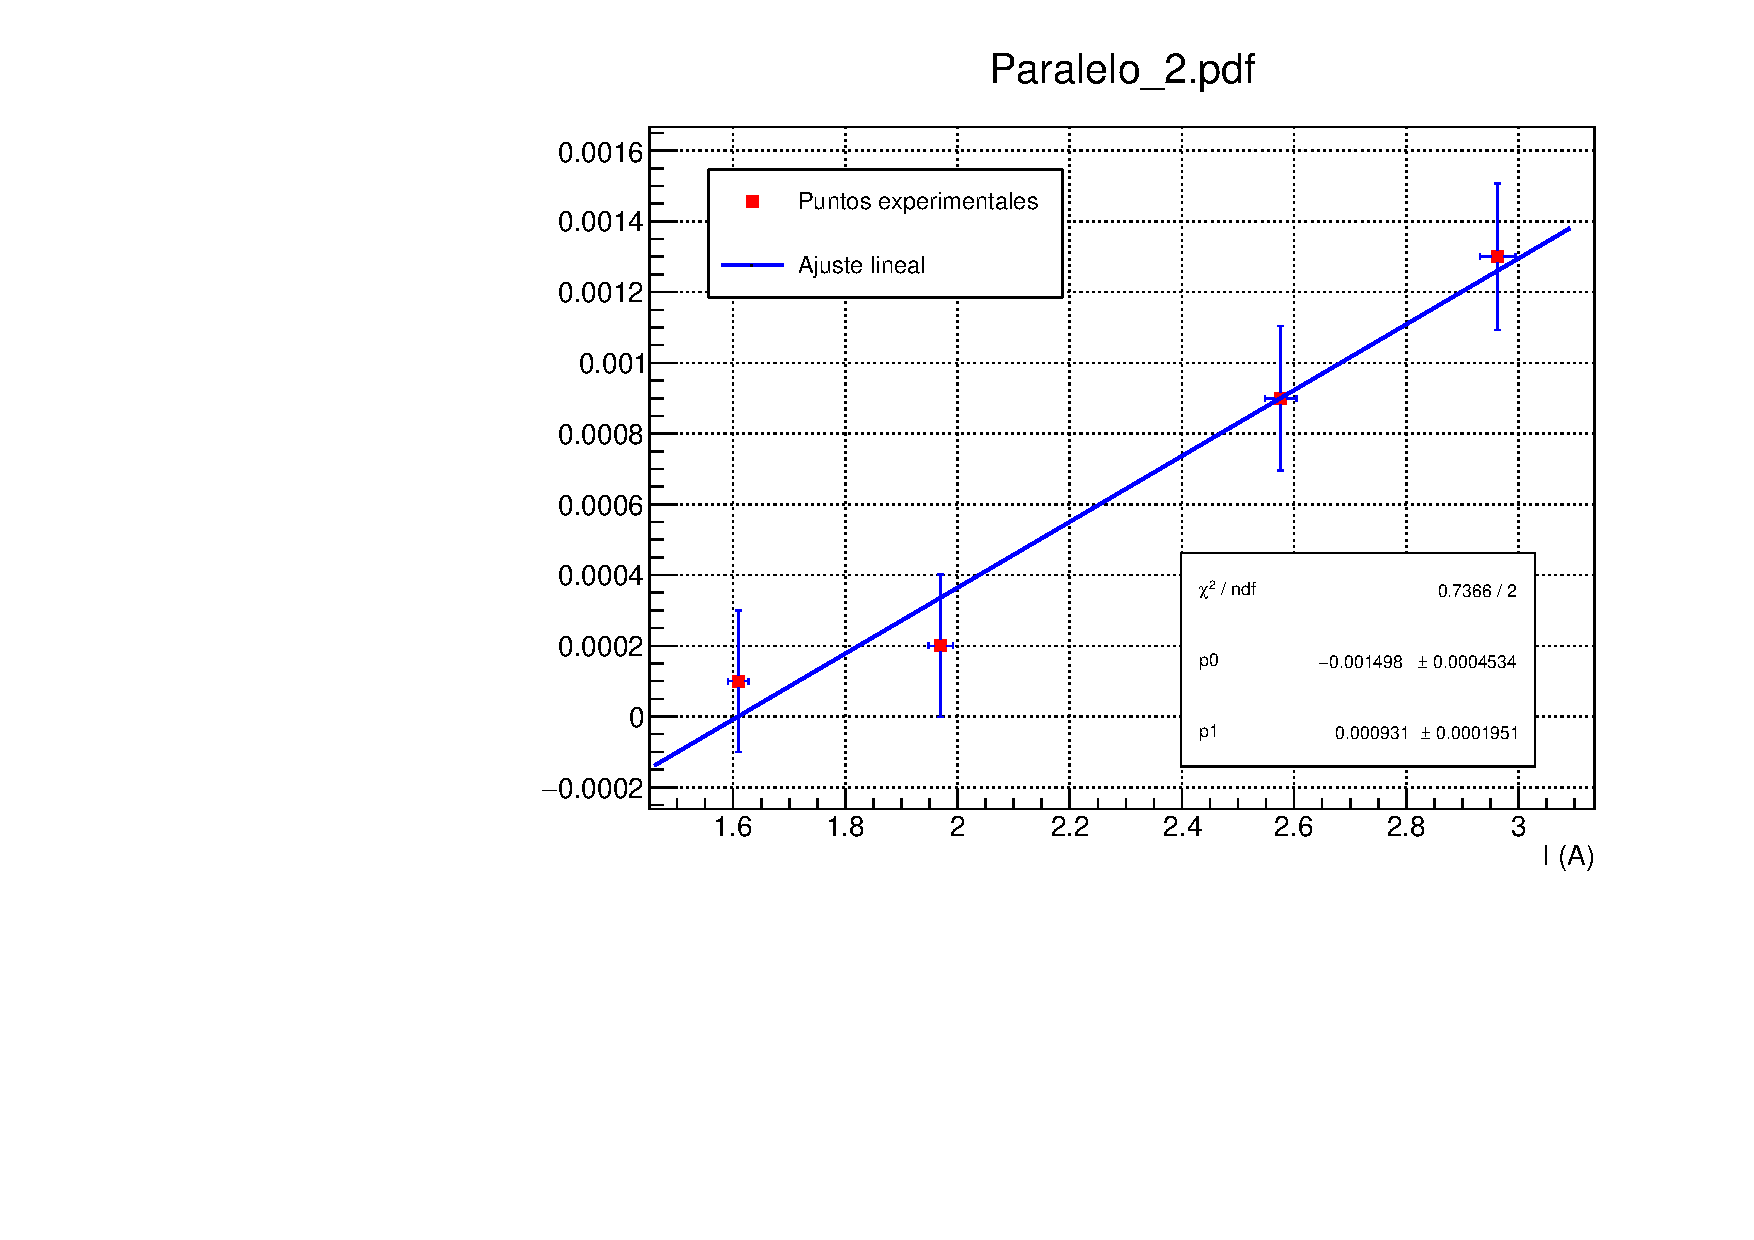
\includegraphics[width=1.05\linewidth]{Programas/Paralelo_2.pdf}
	\end{subfigure}
\end{figure}

Los valores experimentales tal que $\Delta V_{\exp}$, $I_{\exp}$ y $J_{\exp}$, usando que $r=$ tenemos: 

\begin{table}[h!]
    \centering
\begin{tabular}{ccc}
\toprule
$I$ [A] & $V$ [mV] & $J$ [A/cm$^2$] \\
\midrule
2.963 & 0.0013 & 15.057 \\
\bottomrule
\end{tabular}
    \caption{Tabla de la valores para la disposición 4 con $r=0.313$ cm}
    \label{Tab:VIJ_mini_4}
\end{table}


Dado que no podemos calcualr directamente $\Delta V_{\simu}$ ya que alrededor de las terminales varía un poco el voltaje (véase imagen) tal que mediremos varios $V_+$ y $V_-$ simulados, obteniendo una media (y su incertidumbre) y así $\Delta V_{\simu} = \overline{V}_+ - \overline{V}_{-} $. Así pues: \\[1em]

Tal que $\Delta V_{\simu}$ es: \\[1em]

y luego, el valor de la resistividad es:

	

\subsection{Disposición 5}

\begin{figure}[h!]\centering
\begin{subfigure}[b]{0.49\textwidth}
	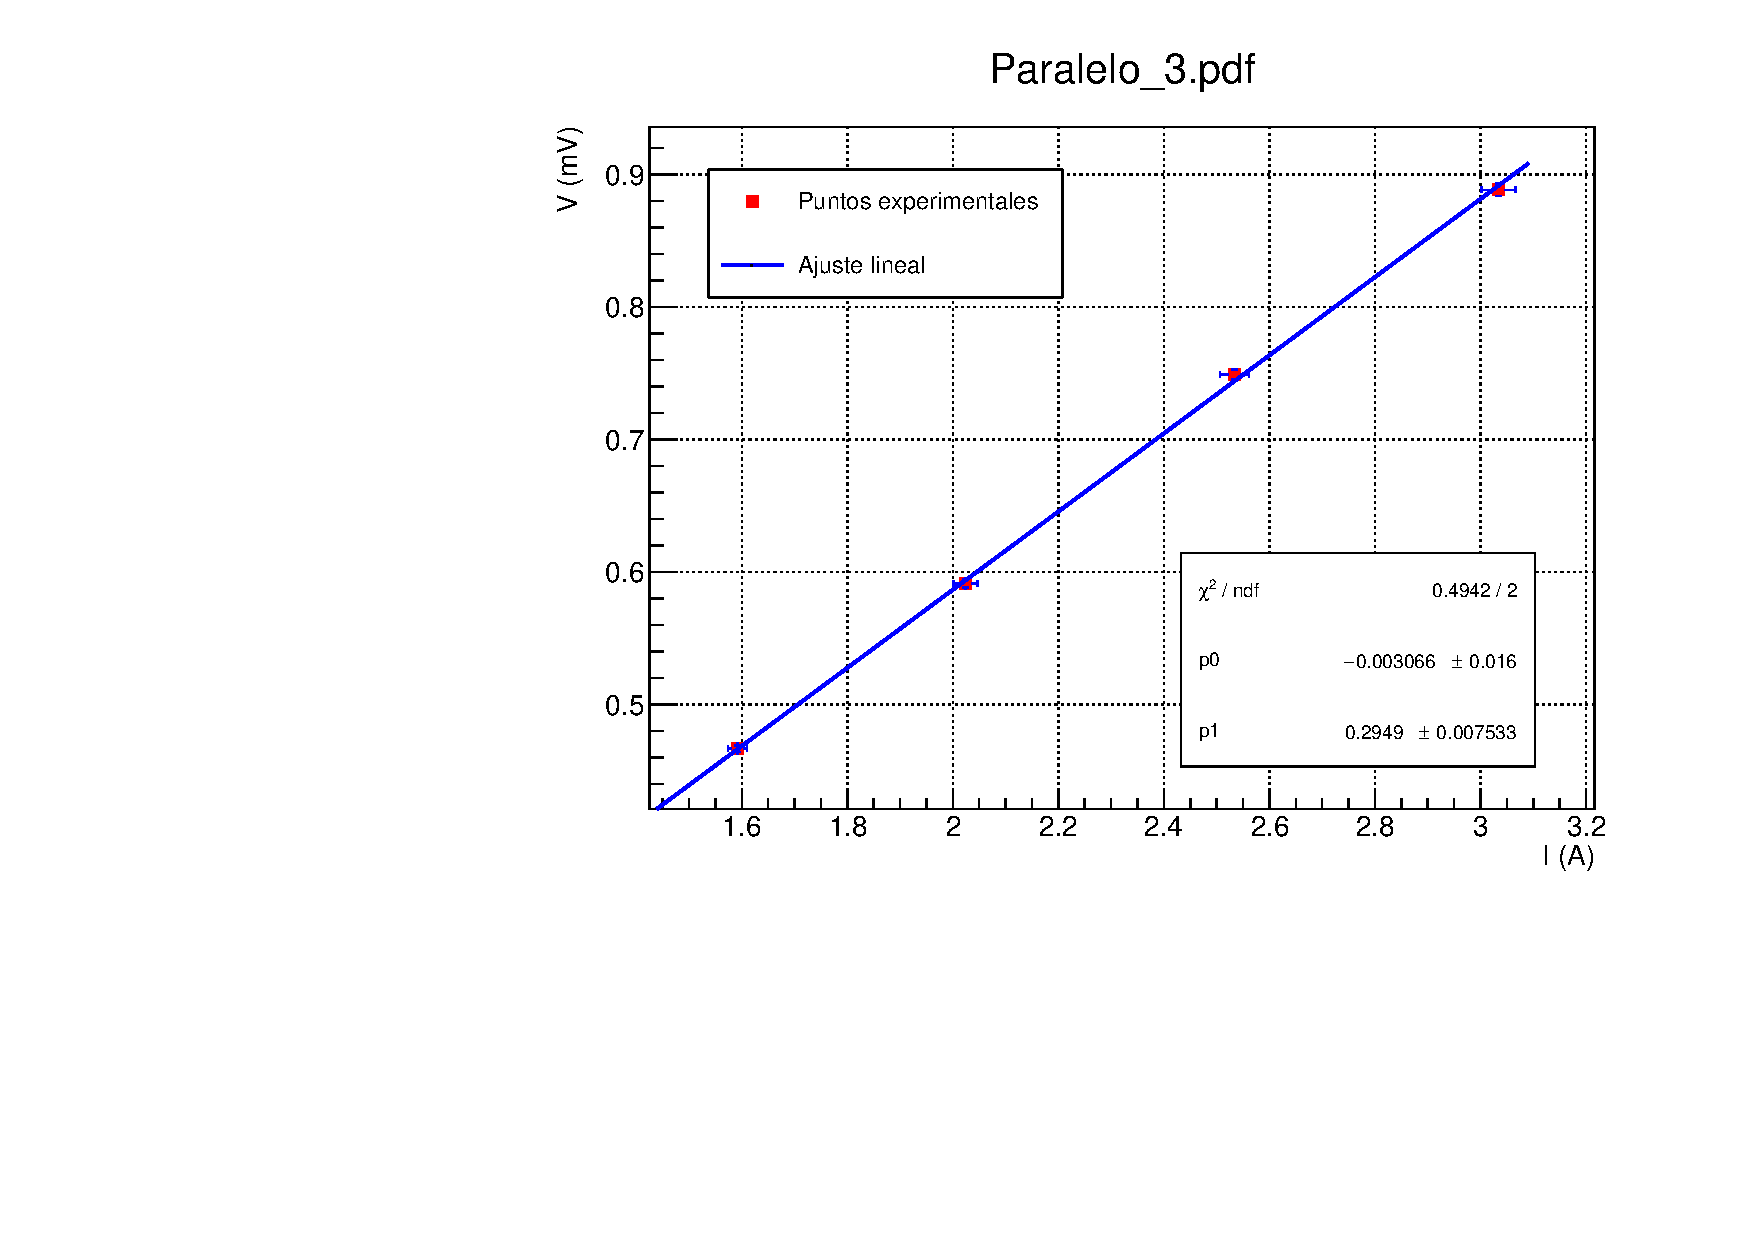
\includegraphics[width=1.05\linewidth]{Programas/Paralelo_3.pdf}
\end{subfigure} \hfill
\begin{subfigure}[b]{0.49\textwidth}
	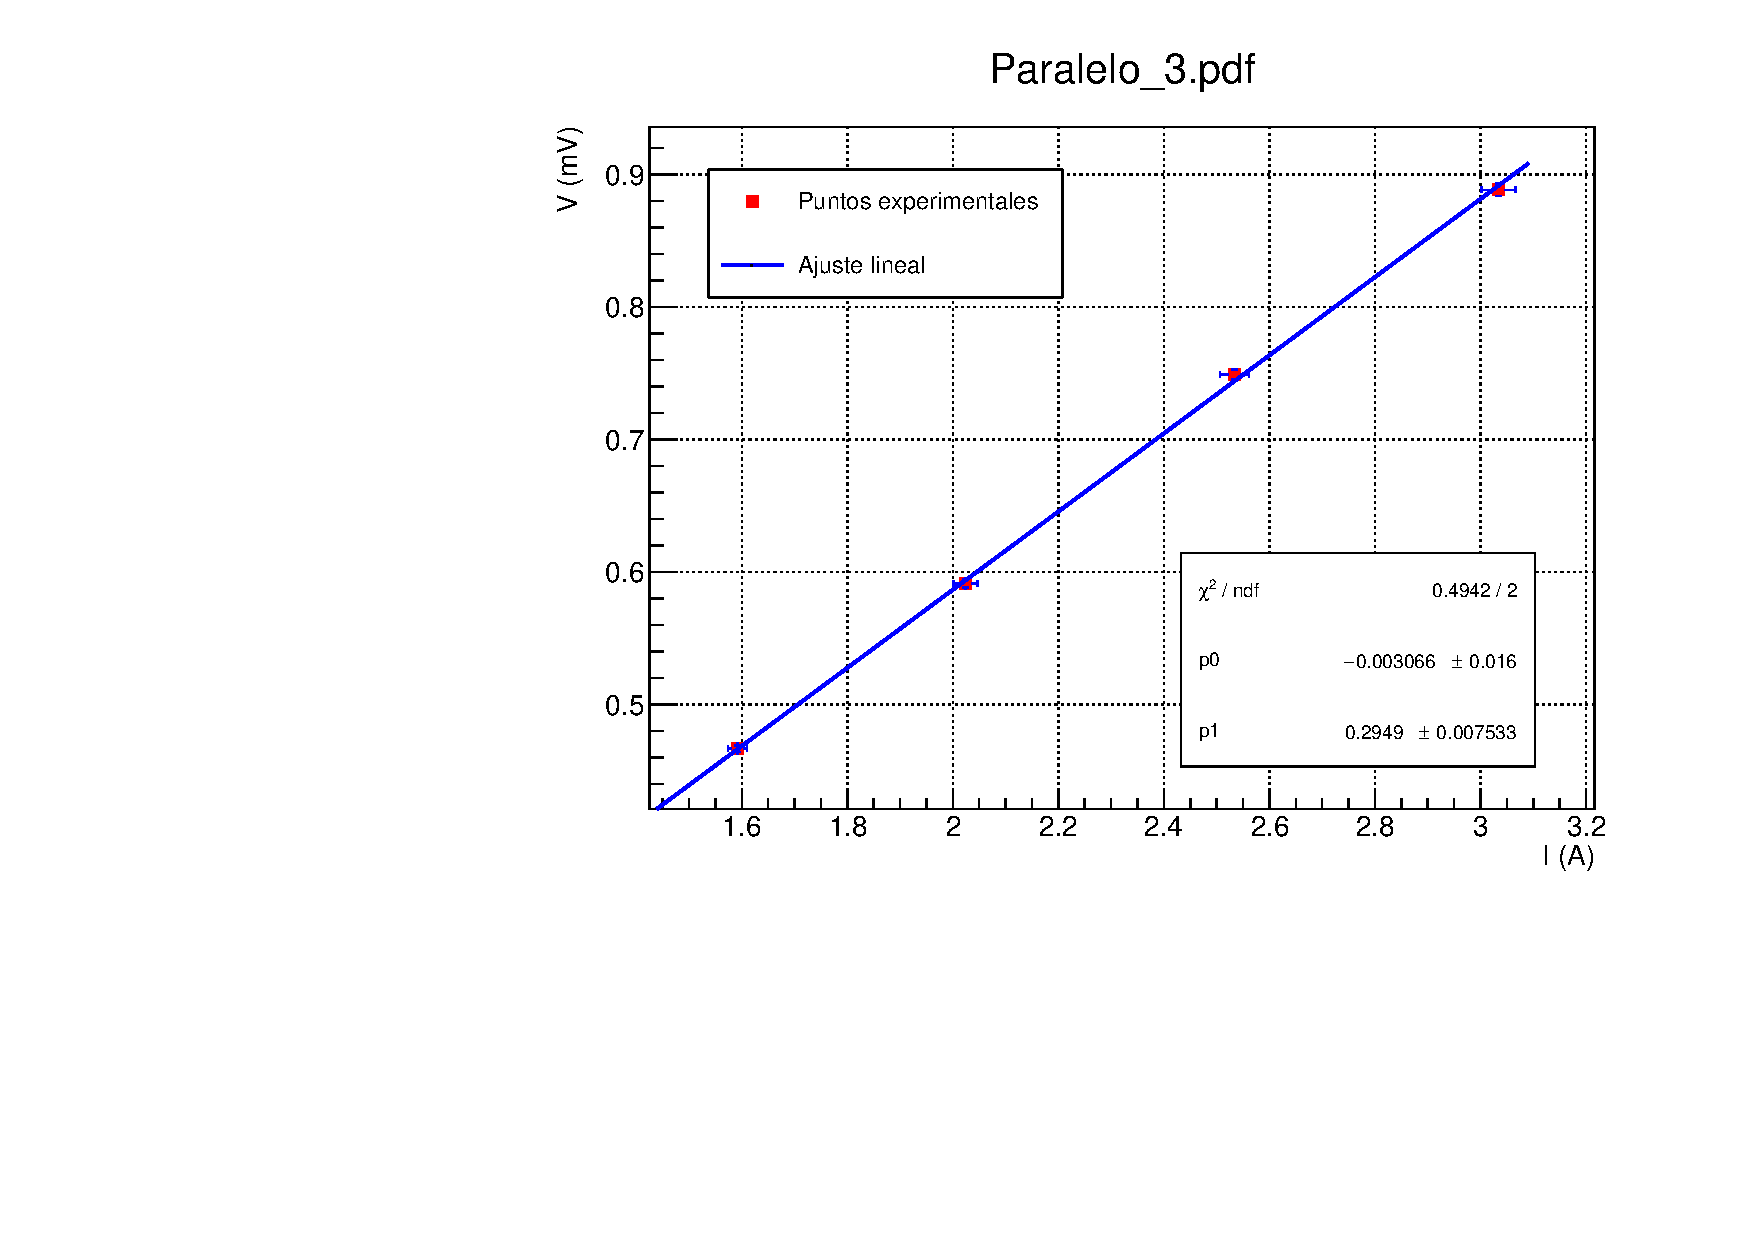
\includegraphics[width=1.05\linewidth]{Programas/Paralelo_3.pdf}
\end{subfigure}
\end{figure}


Los valores experimentales tal que $\Delta V_{\exp}$, $I_{\exp}$ y $J_{\exp}$, usando que $r=$ tenemos: 

\begin{table}[h!]
    \centering
\begin{tabular}{ccc}
\toprule
$I$ [A] & $V$ [mV] & $J$ [A/cm$^2$] \\
\midrule
2.963 & 0.8884 & 15.057 \\
\bottomrule
\end{tabular}
    \caption{Tabla de la valores para la disposición 5 con $r=0.313$ cm}
    \label{Tab:VIJ_mini_5}
\end{table}


Dado que no podemos calcualr directamente $\Delta V_{\simu}$ ya que alrededor de las terminales varía un poco el voltaje (véase imagen) tal que mediremos varios $V_+$ y $V_-$ simulados, obteniendo una media (y su incertidumbre) y así $\Delta V_{\simu} = \overline{V}_+ - \overline{V}_{-} $. Así pues: \\[1em]

Tal que $\Delta V_{\simu}$ es: \\[1em]

y luego, el valor de la resistividad es:
\subsection{Disposición 6}

\begin{figure}[h!]\centering
	\begin{subfigure}[b]{0.49\textwidth}
		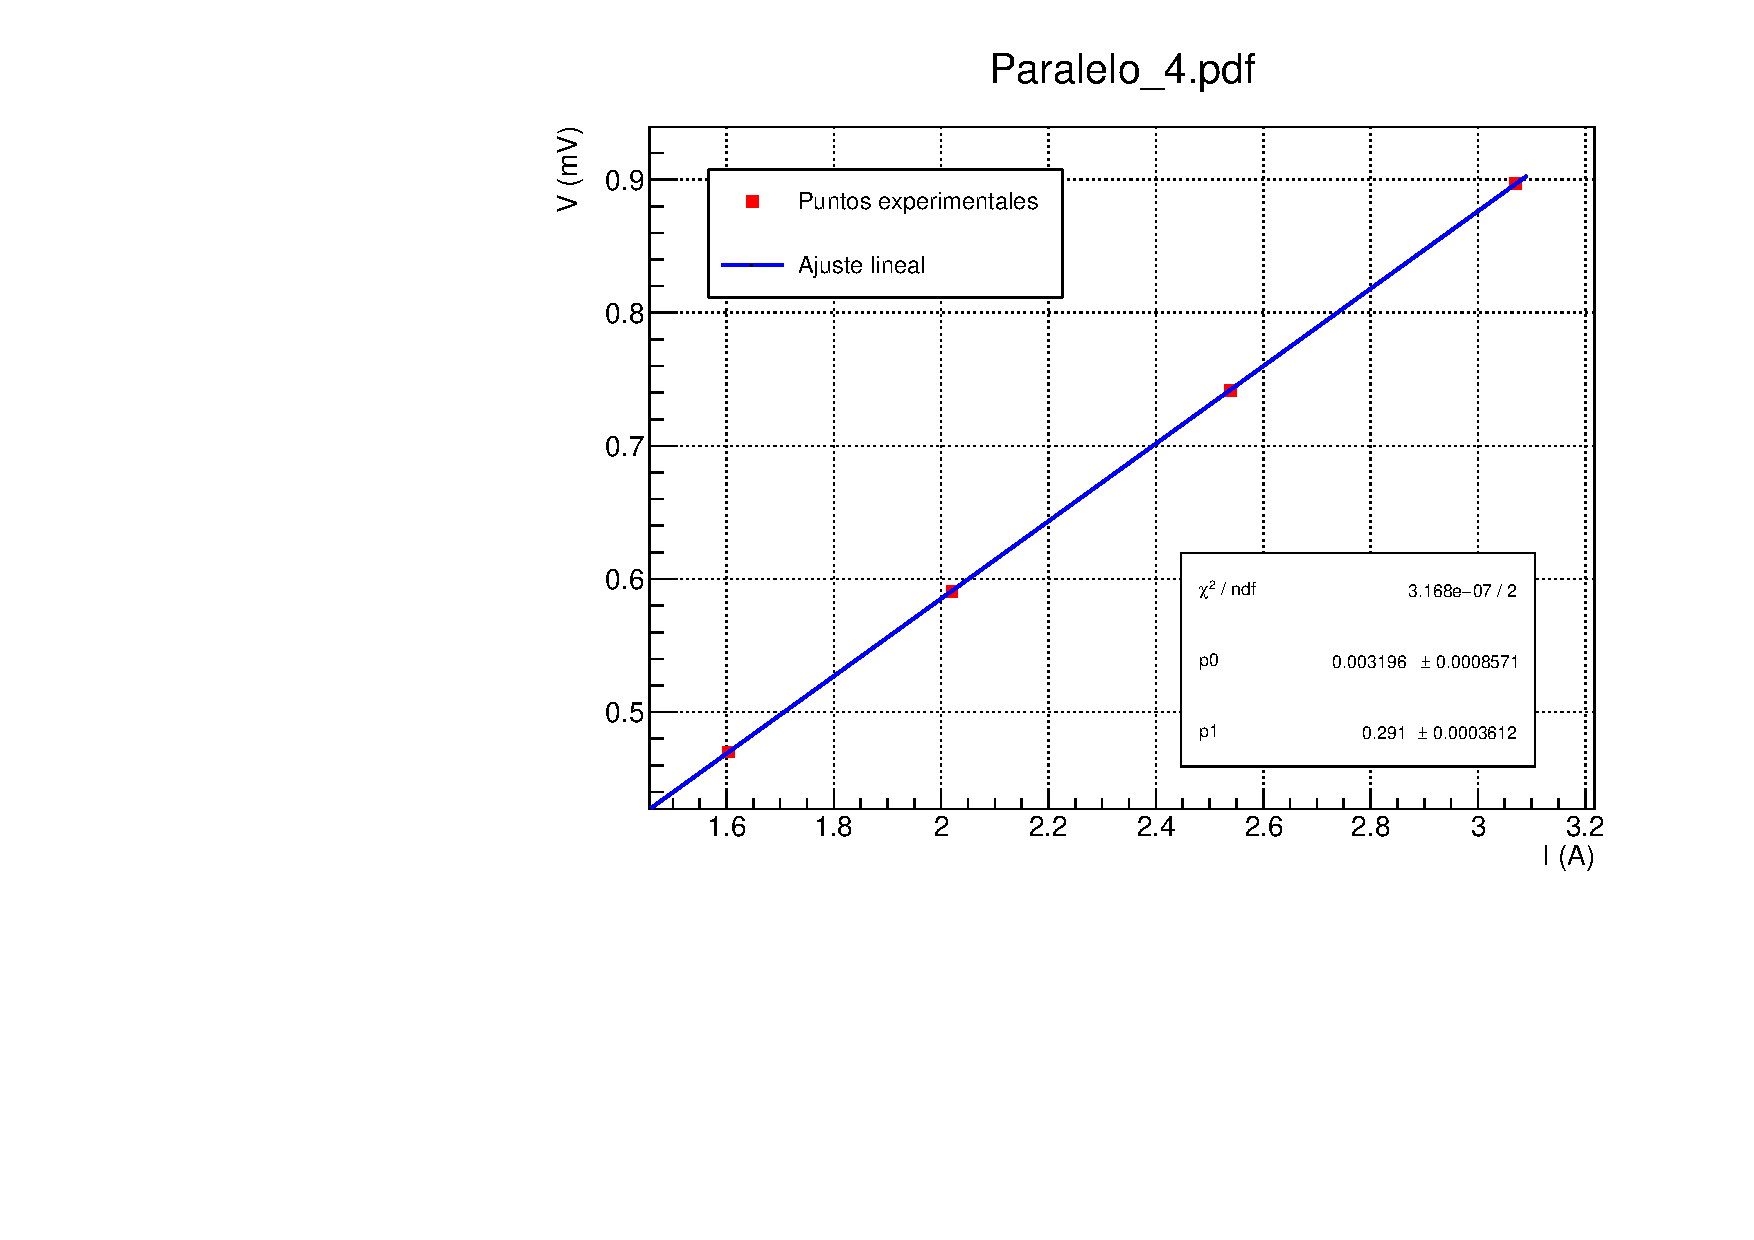
\includegraphics[width=1.05\linewidth]{Programas/Paralelo_4.pdf}
	\end{subfigure} \hfill
	\begin{subfigure}[b]{0.49\textwidth}
		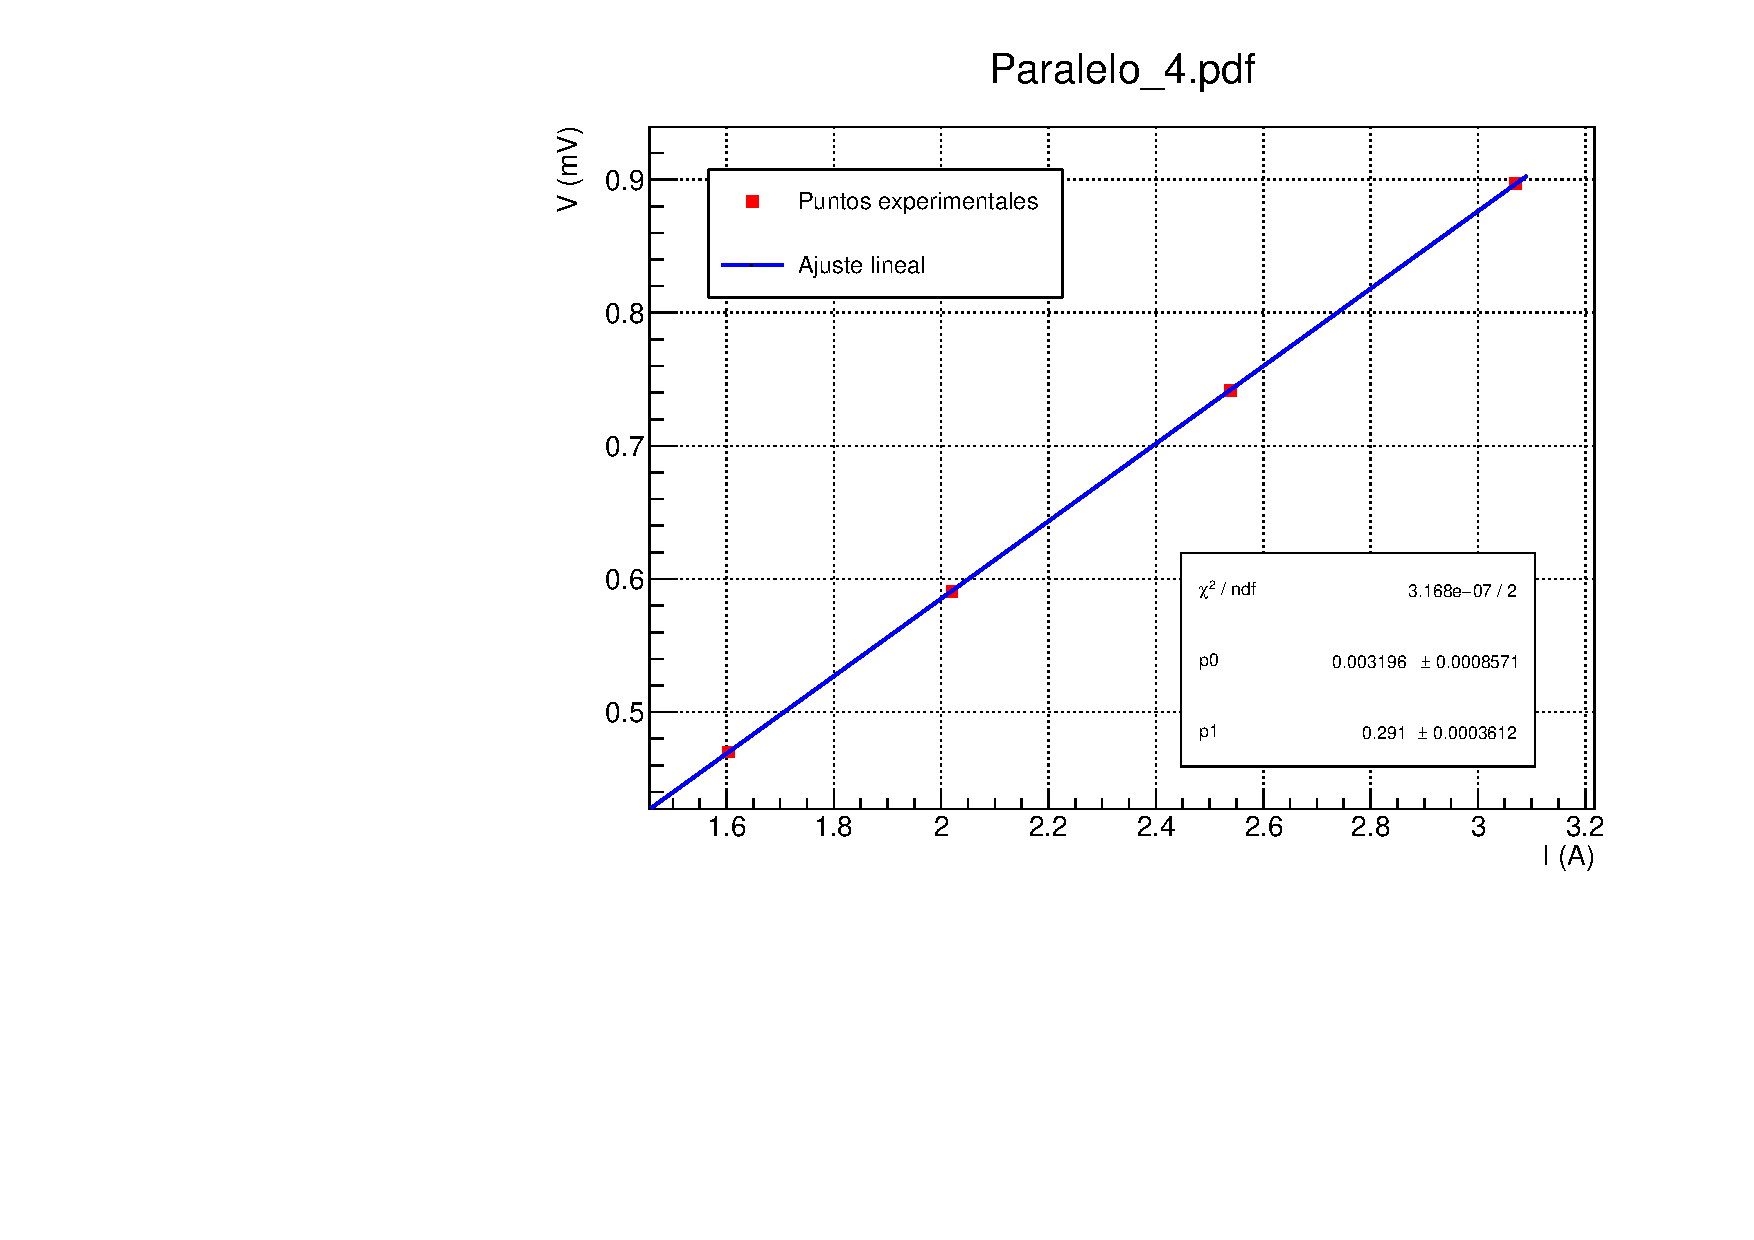
\includegraphics[width=1.05\linewidth]{Programas/Paralelo_4.pdf}
	\end{subfigure}
\end{figure}
	
Los valores experimentales tal que $\Delta V_{\exp}$, $I_{\exp}$ y $J_{\exp}$, usando que $r=$ tenemos: 

\begin{table}[h!]
    \centering
\begin{tabular}{ccc}
\toprule
$I$ [A] & $V$ [mV] & $J$ [A/cm$^2$] \\
\midrule
3.070 & 0.8969 & 15.600 \\
\bottomrule
\end{tabular}
    \caption{Tabla de la valores para la disposición 6 con $r=0.313$ cm}
    \label{Tab:VIJ_mini_6}
\end{table}


Dado que no podemos calcualr directamente $\Delta V_{\simu}$ ya que alrededor de las terminales varía un poco el voltaje (véase imagen) tal que mediremos varios $V_+$ y $V_-$ simulados, obteniendo una media (y su incertidumbre) y así $\Delta V_{\simu} = \overline{V}_+ - \overline{V}_{-} $. 
\newpage

\subsection{Comparación de los valores de la resistividad}

Para calcular los valores de la resistividad, tal y como hemos dicho, tenemos que realizar varias simulaciones en cada uno de los casos, obteniendo 6 valores de la resisitividad. En principio $\sigma \neq \sigma (V)$, por lo que podríamos coger cualquier valor de $V$ para cada una de las simulaciones. En la siguiente tabla presentamos cada uno de los valores que vamos a coger de $V$, $I$, $J$ y $\sigma$, en función de la disposición: 



\newpage

\subsection{¿Dependencia con la disposición?}

En esta seccińo vamos a ver como cambia la resistividad con ciertos valores de la resistividad.

\newpage

\subsection{¿Dependencia con el voltaje?}

En esta sección vamos a estudiar la resistividad con diferentes valores del voltaje. 



\newpage

\section{Conclusiones}


\newpage


\appendix

\section{Tablas:}


\begin{table}[h!]
    \centering
\begin{tabular}{ccc}
\toprule
$I$ [A] & $V$ [mV] & $J$ [A/cm$^2$] \\
\midrule
1.593 & 0.4624 & 8.095 \\
1.984 & 0.5748 & 10.082 \\
2.486 & 0.7210 & 12.633 \\
2.988 & 0.8660 & 15.184 \\
\bottomrule
\end{tabular}
    \caption{Tabla de la valores para la disposición 1 con $r=0.313$ cm}
    \label{Tab:VIJ_1}
\end{table}

\begin{table}[h!]
    \centering
\begin{tabular}{ccc}
\toprule
$I$ [A] & $V$ [mV] & $J$ [A/cm$^2$] \\
\midrule
1.576 & 0.4570 & 8.009 \\
1.979 & 0.5733 & 10.056 \\
2.486 & 0.7200 & 12.633 \\
2.986 & 0.8648 & 15.174 \\
\bottomrule
\end{tabular}
    \caption{Tabla de la valores para la disposición 2 con $r=0.313$ cm}
    \label{Tab:VIJ_2}
\end{table}

\begin{table}[h!]
    \centering
\begin{tabular}{ccc}
\toprule
$I$ [A] & $V$ [mV] & $J$ [A/cm$^2$] \\
\midrule
1.575 & 0.0009 & 8.003 \\
2.020 & 0.0014 & 10.265 \\
2.490 & 0.0017 & 12.653 \\
3.051 & 0.0022 & 15.504 \\
\bottomrule
\end{tabular}
    \caption{Tabla de la valores para la disposición 3 con $r=0.313$ cm}
    \label{Tab:VIJ_3}
\end{table}

\begin{table}[h!]
    \centering
\begin{tabular}{ccc}
\toprule
$I$ [A] & $V$ [mV] & $J$ [A/cm$^2$] \\
\midrule
1.609 & 0.0001 & 8.176 \\
1.970 & 0.0002 & 10.011 \\
2.576 & 0.0009 & 13.090 \\
2.963 & 0.0013 & 15.057 \\
\bottomrule
\end{tabular}
    \caption{Tabla de la valores para la disposición 4 con $r=0.313$ cm}
    \label{Tab:VIJ_4}
\end{table}

\begin{table}[h!]
    \centering
\begin{tabular}{ccc}
\toprule
$I$ [A] & $V$ [mV] & $J$ [A/cm$^2$] \\
\midrule
1.592 & 0.4667 & 8.090 \\
1.970 & 0.5915 & 10.011 \\
2.576 & 0.7491 & 13.090 \\
2.963 & 0.8884 & 15.057 \\
\bottomrule
\end{tabular}
    \caption{Tabla de la valores para la disposición 5 con $r=0.313$ cm}
    \label{Tab:VIJ_5}
\end{table}

\begin{table}[h!]
    \centering
\begin{tabular}{ccc}
\toprule
$I$ [A] & $V$ [mV] & $J$ [A/cm$^2$] \\
\midrule
1.603 & 0.4700 & 8.146 \\
2.020 & 0.5908 & 10.265 \\
2.539 & 0.7418 & 12.902 \\
3.070 & 0.8969 & 15.600 \\
\bottomrule
\end{tabular}
    \caption{Tabla de la valores para la disposición 6 con $r=0.313$ cm}
    \label{Tab:VIJ_6}
\end{table}


\newpage


\newpage


\section{Disposiciones}

\begin{figure}[h!]
\begin{center}
\begin{tikzpicture}
	\node at (0,0) {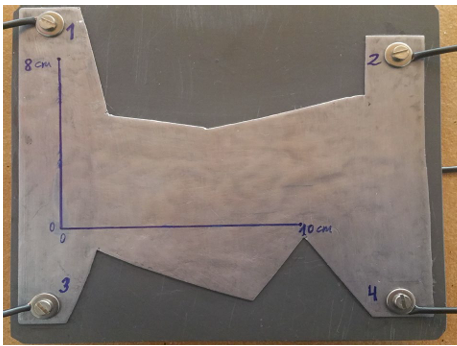
\includegraphics[width=0.8\linewidth]{Agros/placa prueba.png}};
	
  \draw[fill=red] (4.5,3.2) circle  (0.35cm);
  \node at (4.5,3.2) {\textcolor{white}{$\mathbf{I^+}$}};

  \draw[fill=black] (4.6,-3.3) circle  (0.35cm);
  \node at (4.6,-3.3) {\textcolor{white}{$\mathbf{V^+}$}};

  \draw[fill=black!50!white] (-4.9,3.9) circle (0.35cm);
  \node at (-4.9,3.9) {\textcolor{white}{$\mathbf{V^-}$}};

  \draw[fill=blue] (-4.9,-3.5) circle (0.35cm);
  \node at (-4.9,-3.5) {\textcolor{white}{$\mathbf{I^-}$}};
\end{tikzpicture}
\end{center}
\caption{Primera disposición usada: cruzada 1.}
\end{figure}

\begin{figure}[h!]
\begin{center}
	\begin{tikzpicture}
		\node at (0,0) {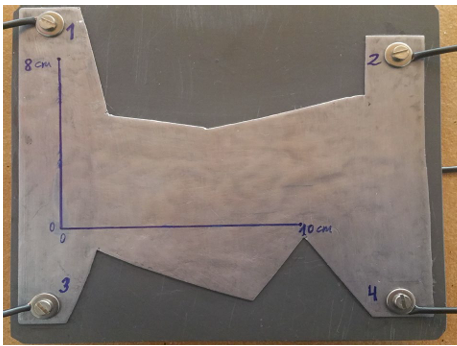
\includegraphics[width=0.8\linewidth]{Agros/placa prueba.png}};
		
	  \draw[fill=black] (4.5,3.2) circle  (0.35cm);
	  \node at (4.5,3.2) {\textcolor{white}{$\mathbf{V^+}$}};
	
	  \draw[fill=red] (4.6,-3.3) circle  (0.35cm);
	  \node at (4.6,-3.3) {\textcolor{white}{$\mathbf{I^+}$}};
	
	  \draw[fill=blue] (-4.9,3.9) circle (0.35cm);
	  \node at (-4.9,3.9) {\textcolor{white}{$\mathbf{I^-}$}};
	
	  \draw[fill=black!50!white] (-4.9,-3.5) circle (0.35cm);
	  \node at (-4.9,-3.5) {\textcolor{white}{$\mathbf{V^-}$}};
	\end{tikzpicture}
	\end{center}
	\caption{Segunda disposición usada: cruzada 2.}
\end{figure}

\newpage


\begin{figure}[h!]
	\begin{center}
		\begin{tikzpicture}
			\node at (0,0) {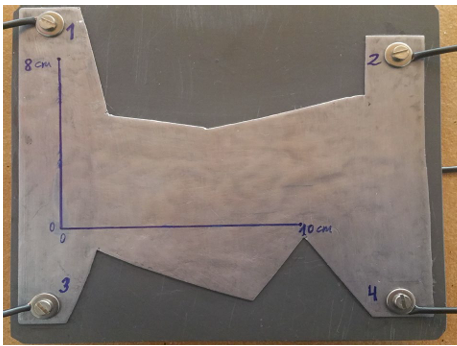
\includegraphics[width=0.8\linewidth]{Agros/placa prueba.png}};
			
		  \draw[fill=black!50!white] (4.5,3.2) circle  (0.35cm);
		  \node at (4.5,3.2) {\textcolor{white}{$\mathbf{V^-}$}};
		
		  \draw[fill=black] (4.6,-3.3) circle  (0.35cm);
		  \node at (4.6,-3.3) {\textcolor{white}{$\mathbf{V^+}$}};
		
		  \draw[fill=blue] (-4.9,3.9) circle (0.35cm);
		  \node at (-4.9,3.9) {\textcolor{white}{$\mathbf{I^-}$}};
		
		  \draw[fill=red] (-4.9,-3.5) circle (0.35cm);
		  \node at (-4.9,-3.5) {\textcolor{white}{$\mathbf{I^+}$}};
		\end{tikzpicture}
		\end{center}
		\caption{Tercera disposición usada: paralela 1.}
	\end{figure}

	

\begin{figure}[h!]
	\begin{center}
		\begin{tikzpicture}
			\node at (0,0) {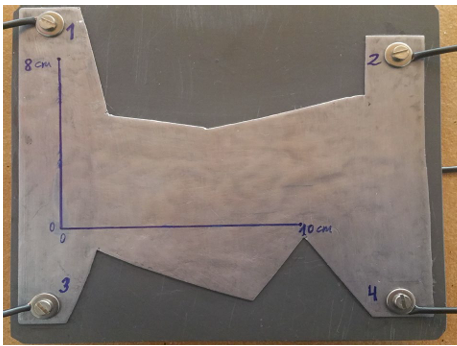
\includegraphics[width=0.8\linewidth]{Agros/placa prueba.png}};
			
		  \draw[fill=red] (4.5,3.2) circle  (0.35cm);
		  \node at (4.5,3.2) {\textcolor{white}{$\mathbf{I^+}$}};
		
		  \draw[fill=blue] (4.6,-3.3) circle  (0.35cm);
		  \node at (4.6,-3.3) {\textcolor{white}{$\mathbf{I^-}$}};
		
		  \draw[fill=black] (-4.9,3.9) circle (0.35cm);
		  \node at (-4.9,3.9) {\textcolor{white}{$\mathbf{V^+}$}};
		
		  \draw[fill=black!50!white] (-4.9,-3.5) circle (0.35cm);
		  \node at (-4.9,-3.5) {\textcolor{white}{$\mathbf{V^-}$}};
		\end{tikzpicture}
		\end{center}
		\caption{Cuarta disposición usada: paralela 2.}
\end{figure}

\newpage

\begin{figure}[h!]
	\begin{center}
		\begin{tikzpicture}
			\node at (0,0) {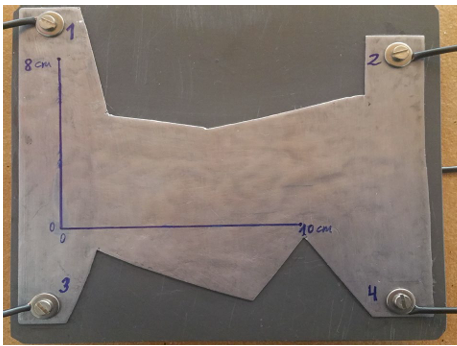
\includegraphics[width=0.8\linewidth]{Agros/placa prueba.png}};
			
		  \draw[fill=red] (4.5,3.2) circle  (0.35cm);
		  \node at (4.5,3.2) {\textcolor{white}{$\mathbf{I^+}$}};
		
		  \draw[fill=black!50!white] (4.6,-3.3) circle  (0.35cm);
		  \node at (4.6,-3.3) {\textcolor{white}{$\mathbf{V^-}$}};
		
		  \draw[fill=blue] (-4.9,3.9) circle (0.35cm);
		  \node at (-4.9,3.9) {\textcolor{white}{$\mathbf{I^-}$}};
		
		  \draw[fill=black] (-4.9,-3.5) circle (0.35cm);
		  \node at (-4.9,-3.5) {\textcolor{white}{$\mathbf{V^+}$}};
		\end{tikzpicture}
		\end{center}
		\caption{Quinta disposición usada: paralela 3.}
\end{figure}
	


\begin{figure}[h!]
	\begin{center}
		\begin{tikzpicture}
			\node at (0,0) {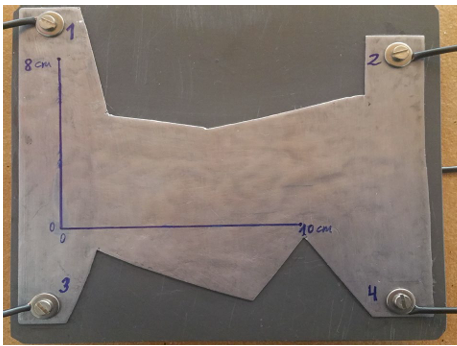
\includegraphics[width=0.8\linewidth]{Agros/placa prueba.png}};
			
		  \draw[fill=black!50!white] (4.5,3.2) circle  (0.35cm);
		  \node at (4.5,3.2) {\textcolor{white}{$\mathbf{V^-}$}};
		
		  \draw[fill=red] (4.6,-3.3) circle  (0.35cm);
		  \node at (4.6,-3.3) {\textcolor{white}{$\mathbf{I^+}$}};
		
		  \draw[fill=black] (-4.9,3.9) circle (0.35cm);
		  \node at (-4.9,3.9) {\textcolor{white}{$\mathbf{V^+}$}};
		
		  \draw[fill=blue] (-4.9,-3.5) circle (0.35cm);
		  \node at (-4.9,-3.5) {\textcolor{white}{$\mathbf{I^-}$}};
		\end{tikzpicture}
		\end{center}
		\caption{Sexta disposición usada: paralela 4.}
\end{figure}
	

\newpage

	
\printbibliography

	



\end{document}